\newpage
\section{Appendix}
\appendix

\label{appendix}

\section{Datasets}
\label{appendix:data}

Here we list all of the datasets with their corresponding information (Tab.~\ref{tab:datasets}). We used eight classification and eight regression datasets. For each dataset, we list the number of samples, the number of features, the distribution of the target variable, and a link to the dataset.

\begin{table}[hbt]
    \centering
    \begin{tabular}{p{0.03\textwidth}|c|r|r|r|c}
        \centering \textbf{} & \raggedright \textbf{dataset} & \raggedright\arraybackslash \textbf{Samples} & \raggedright\arraybackslash \textbf{Features} & \raggedright\arraybackslash \textbf{Target} & \raggedright\arraybackslash \textbf{Link} \\
        \hline 
        \parbox[t]{3mm}{\multirow{8}{*}{\rotatebox[origin=c]{90}{Classification}}}
        & Heart & 270 & 15 & $44.4\%$ & \href{https://archive.ics.uci.edu/ml/datasets/Statlog+%28Heart%29}{UCI ML repo} \\
        & Breast cancer & 286 & 9 & $29.2\%$ & \href{https://archive.ics.uci.edu/ml/datasets/Breast+Cancer+Wisconsin+%28Original%29}{UCI ML repo} \\
        & Haberman & 306 & 3 & $73.5\%$ & \href{https://archive.ics.uci.edu/ml/datasets/Haberman%27s+Survival}{UCI ML repo} \\
        & Ionosphere & 351 & 34 & $64.1\%$ & \href{https://archive.ics.uci.edu/ml/datasets/Ionosphere}{UCI ML repo} \\
        & Diabetes & 768 & 8 & $34.9\%$ & \href{https://www.kaggle.com/datasets/mathchi/diabetes-data-set}{Kaggle} \\
        & German credit & 1000 & 20 & $70.0\%$ & \href{https://archive.ics.uci.edu/ml/datasets/South+German+Credit+%28UPDATE%29}{UCI ML repo} \\
        & Juvenile & 3640 & 286 & $13.4\%$ & \href{https://www.icpsr.umich.edu/web/NACJD/studies/3986}{nacjd} \\
        & Recidivism & 6172 & 20 & $48.4\%$ & \href{https://www.propublica.org/datastore/dataset/compas-recidivism-risk-score-data-and-analysis}{ProPublica} \\
        \hline
        \parbox[t]{4mm}{\multirow{8}{*}{\rotatebox[origin=c]{90}{Regression}}} 
        & Friedman1 & 200 & 10 & $ 14.25 \pm 5.01 $ & \href{https://scikit-learn.org/stable/modules/generated/sklearn.datasets.make_friedman1.html}{scikit-learn} \\
        & Friedman3 & 200 & 4 & $ 1.33 \pm 0.30 $ & \href{https://scikit-learn.org/stable/modules/generated/sklearn.datasets.make_friedman3.html}{scikit-learn} \\
        & Diabetes & 442 & 10 & $ 152.1 \pm 77.1 $ & \href{https://scikit-learn.org/stable/modules/generated/sklearn.datasets.load_diabetes.html}{scikit-learn} \\
        & Geographical music & 1059 & 117 & $ 0.02 \pm 1.00 $ & \href{https://epistasislab.github.io/pmlb/profile/4544_GeographicalOriginalofMusic.html}{PMLB} \\
        & Red wine & 1599 & 11 & $ 5.63 \pm 0.81 $ & \href{https://archive.ics.uci.edu/ml/datasets/Wine+Quality}{UCI ML repo} \\
        & Abalone & 4177 & 8 & $ 9.93 \pm 3.22 $ & \href{https://archive.ics.uci.edu/ml/datasets/Abalone}{UCI ML repo} \\
        & Satellite image & 6435 & 36 & $ 3.67 \pm 2.21 $ & \href{https://epistasislab.github.io/pmlb/profile/294_satellite_image.html}{PMLB} \\
        & CA housing & 20640 & 8 & $ 2.07 \pm 1.15 $ & \href{https://www.kaggle.com/datasets/camnugent/california-housing-prices}{Kaggle} \\
        \hline
    \end{tabular}
    \caption{Datasets used by the authors throughout their paper. The Target column displays the percentage of positive cases for classification tasks, and mean response value with standard deviation for regression tasks.}
    \label{tab:datasets}
\end{table}

\section{Claim 1: HS increases the predictive power of TBM.}
\label{appendix:claim1}
% the \\ insures the section title is centered below the phrase: AppendixA

Based on Fig~\ref{fig:apendix-fig4-claim1} we can see that our results are similar in terms of mean score to the original paper, the only consistent difference being the larger variance. 
This explains the observed disparity between ours and the author's results since while HS-DT performs better than DT, the difference is not statistically significant\footnote{We considered differences statistically significant if they differed by one standard deviation.} due to the larger variance.

\begin{figure}[hbt]
    \centering
    \begin{subfigure}[b]{\textwidth}
        \centering
        \includegraphics[width=\textwidth]{images/appendix/claim1/classification_dt_1.png}
        \caption{DT $AUC$ score before and after applying HS regularization.}
    \end{subfigure}
    \vspace{-1em}
    
    \begin{subfigure}[b]{\textwidth}
        \centering
        \includegraphics[width=\textwidth]{images/appendix/claim1/regression_dt_1.png}
        \caption{DT $R^2$ score before and after applying HS regularization.}
    \end{subfigure}
    \vspace{-1em}
    
    \begin{subfigure}[b]{\textwidth}
        \centering
        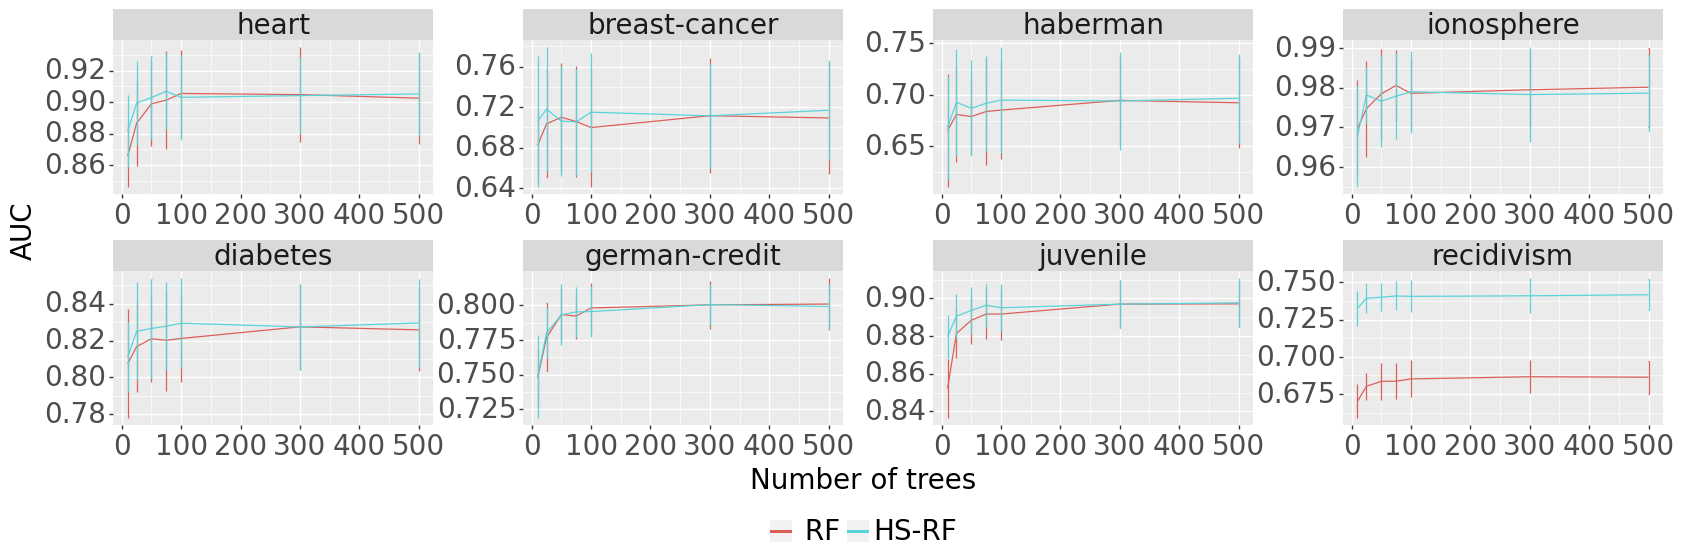
\includegraphics[width=\textwidth]{images/appendix/claim1/classification_rf_1.png}
        \caption{RF $AUC$ score before and after applying HS regularization.}
    \end{subfigure}
    \caption{HS improves DT $AUC$ and $R^2$ score for smaller datasets with the improvements decreasing as the dataset size grows, however for RF no such improvement is visible.}
    \label{fig:apendix-fig4-claim1}
\end{figure}

We further analyzed the likelihood that the top scores of HS-DT were better than the top DT scores (Fig.~\ref{fig:apendix-fig4-top}) and found this to be the case in nearly all instances with improvements being less pronounced for regression than for classification. 
This might indicate that HS influences different evaluation metrics differently.

\begin{figure}[hbt]
    \centering
    \begin{subfigure}[b]{\textwidth}
        \begin{subfigure}[b]{0.48\textwidth}
            \centering
            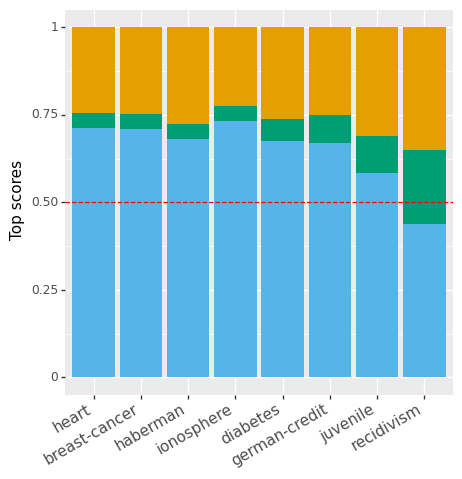
\includegraphics[width=\textwidth]{images/appendix/claim1/DT-top-class-likelihood.png}
        \end{subfigure}
        \begin{subfigure}[b]{0.45\textwidth}
            \centering
            \includegraphics[width=\textwidth]{images/appendix/claim1/DT-top-reg-likelihood.png}
        \end{subfigure}
        \caption{Comparison of top scores between HS-DT and DT for each dataset.}
        \label{fig:apendix-fig4-top}
    \end{subfigure}
    
    \begin{subfigure}[b]{\textwidth}
        \begin{subfigure}[b]{0.48\textwidth}
            \centering
            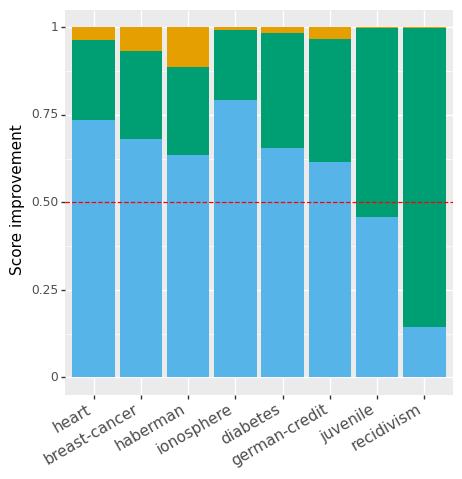
\includegraphics[width=\textwidth]{images/appendix/claim1/DT-any-class-likelihood.png}
        \end{subfigure}
        \begin{subfigure}[b]{0.45\textwidth}
            \centering
            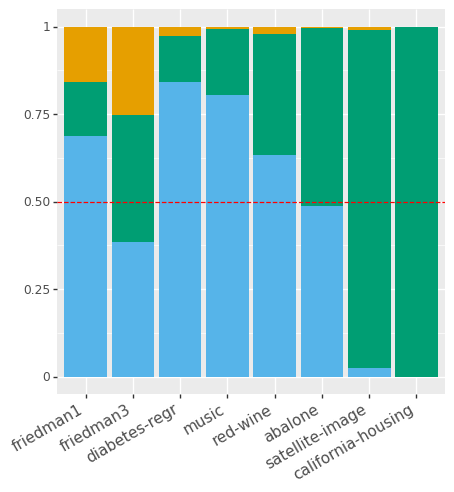
\includegraphics[width=\textwidth]{images/appendix/claim1/DT-any-reg-likelihood.png}
        \end{subfigure}
        \caption{Comparison of improvement in DT scores before and after HS regularization for each dataset.}
        \label{fig:apendix-fig4-any}
    \end{subfigure}
    
    \begin{subfigure}[b]{\textwidth}
        \begin{subfigure}[b]{0.48\textwidth}
            \centering
            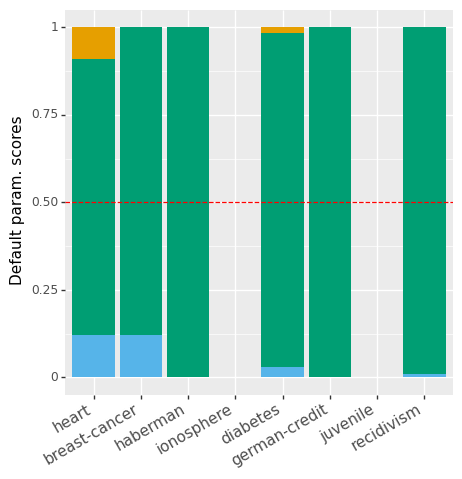
\includegraphics[width=\textwidth]{images/appendix/claim1/DT-heuristic-class-likelihood.png}
        \end{subfigure}
        \begin{subfigure}[b]{0.45\textwidth}
            \centering
            \includegraphics[width=\textwidth]{images/appendix/claim1/DT-heuristic-reg-likelihood.png}
        \end{subfigure}
        \label{fig:apendix-fig4-rf-improvement}
        \caption{Comparison of scores between HS-DT and DT when using default hyperparameters for each dataset.}
    \end{subfigure}
    \caption{Each figure in our image set represents the likelihood that out of 1000 sampled pairs HS scored better (blue), both pairs scored the same (green) or DT scored better (orange).}
\end{figure}

When checking the likelihood of improvement (Fig.~\ref{fig:apendix-fig4-any}) we can see that the likelihood that applying HS to DT improves the scores or does not significantly worsen them is almost $100\%$ indicating that HS is indeed a valid form of regularization for DT.

Finally, we checked how HS improved DT when the DT was trained using the default number of leaves\footnote{Missing bars indicate that DT built less than five trees near the default number of trees making it so that our conclusions would not have enough significance for those datasets.}. This is $n/3$ and $\sqrt{n}$ for regression and classification, respectively.
Here it is apparent that there are no improvements, likely due to the fact that the defaults build small trees that cannot be regularized significantly, therefore users should not expect improvements if they use HS while using default parameters.

\begin{figure}[hbt]
    \begin{subfigure}[b]{\textwidth}
        \begin{subfigure}[b]{0.48\textwidth}
            \centering
            \includegraphics[width=\textwidth]{images/appendix/claim1/RF-top-class-likelihood.png}
            \caption{Comparison of top scores of HS-RF and of RF for each dataset. \label{fig:apendix-fig4-rf-top}}
        \end{subfigure}
        \begin{subfigure}[b]{0.48\textwidth}
            \centering
            \includegraphics[width=\textwidth]{images/appendix/claim1/RF-any-class-likelihood.png}
            \caption{Comparison of improvement in RF scores before and after HS regularization for each dataset. \label{fig:apendix-fig4-rf-imp}}
        \end{subfigure}
    \end{subfigure}
    \caption{Each figure in our image set represents the likelihood that out of 1000 sampled pairs HS scored better (blue), both pairs scored the same (green) or RF scored better (orange).}
\end{figure}

When comparing top scores of HS-RF and RF (Fig.~\ref{fig:apendix-fig4-rf-top}) it appears that the likelihood that we can generate a top score using RF is similar to the likelihood that we can generate a top score using HS-RF indicating that HS does not significantly improve RF scores. This conclusion is enforced by the comparison of RF and RF after HS was applied to it (Fig.~\ref{fig:apendix-fig4-rf-imp}) indicating that while some improvements were still visible these improvements were much smaller and much less consistent across datasets.
We conclude this is likely due to the regularizing effect of using ensembles which decreases the potential improvements offered by HS.

\section{Claim 2: HS is better than other regularization algorithms for TBM.}
\label{appendix:claim2}

In this section, we investigate whether HS is better than other regularization algorithms for TBM. 
Based on our results we conclude that HS is not significantly better than other regularization methods. 
For DT HS-CCP is significantly better than CCP, but not significantly better than LBS (Fig.~\ref{app2-class} \& \ref{app2-reg}\footnote{We did not calculate the experiment for california-housing due to the large execution time of CCP on large datasets; To train one DT regularized with CCP it took approx 1.5 h of wall time (see~Tab.~\ref{tab:app-claim3-dt})}) as the later occasionally performs better and occasionally worse but always within one standard deviation of HS-CCP.

For RF (Fig.~\ref{app2-rf}) we can see that in most instances all methods perform similarly to one another, the exceptions being the breast-cancer and recidivism dataset. 
There is no consistency in how our scores differ from the original papers; for datasets like haberman they are higher, for breast-cancer they are lower and for heart they are roughly the same. 
Based on the above observation and the high variance of scores we conclude that neither our nor the author's results are necessarily conclusive and more samples would need to be generated in order to definitively show which method is better.

\begin{figure}[hbt]
    \centering
    \begin{subfigure}[b]{\textwidth}
        \centering
        \includegraphics[width=\textwidth]{images/appendix/claim2/fig_4_dt-class.png}
        \caption{DT $AUC$ score before and after applying HS regularization. \label{app2-class}}
    \end{subfigure}
    \vspace{-1em}
    
    \begin{subfigure}[b]{\textwidth}
        \centering
        \includegraphics[width=\textwidth]{images/appendix/claim2/fig_4_dt-reg.png}
        \caption{DT $R^2$ score before and after applying HS regularization. \label{app2-reg}}
    \end{subfigure}
    \vspace{-1em}
    
    \begin{subfigure}[b]{\textwidth}
        \centering
        \includegraphics[width=\textwidth]{images/appendix/claim2/fig_4_rf-class.png}
        \caption{RF $AUC$ score before and after applying HS regularization. \label{app2-rf}}
    \end{subfigure}
    \caption{HS improves DT $AUC$ and $R^2$ score for smaller datasets with the improvements decreasing as the dataset size grows, however for RF no such improvement is visible.}
    \label{fig:apendix-fig4-claim2}
\end{figure}

\section{Claim 3: HS is faster than other post-hoc regularization algorithms for TBM.}
\label{appendix:claim3}
% the \\ insures the section title is centered below the phrase: Appendix B

In this section, we investigate the execution time of HS in comparison to other regularization algorithms for DT. 
Based on our results we conclude that as the size of the dataset grows HS the differences in speed become more pronounced with HS becoming significantly faster for larger datasets.
Additionally, it appears that especially for small datasets CCP is faster than HS.
We also note that there appear to be no significant differences between cpu and wall time indicating that parallelization has no impact on the speed of regularization of DT.

% TODO: add regression for DT and RF

\begin{table}[hbt]
    \centering
    \begin{tabular}{|l|c|r|c|r|}
    %\toprule
    %{} & \multicolumn{4}{|c|}{RF} %& \multicolumn{1}{2}{DT} \\
    \toprule
    {} & base & \multicolumn{1}{|c|}{overtime} & base & \multicolumn{1}{|c|}{overtime} \\
    \toprule
    {} &  \makecell{$hs$\\wall} &  \makecell{$ccp$\\wall} &  \makecell{$hs$\\cpu} &  \makecell{$ccp$\\cpu} \\
    dataset       &             &                                                  &          &                                             \\
    \midrule
    heart         &    $0.019$  &      \cellcolor{red!15}$-0.010 \pm \,\,\,0.000$ & $0.019$  & \cellcolor{red!15}$-0.010 \pm \,\,\,0.000$ \\
    breast-cancer &    $0.019$  &      \cellcolor{red!15}$-0.009 \pm \,\,\,0.000$ & $0.019$  & \cellcolor{red!15}$-0.009 \pm \,\,\,0.000$  \\
    haberman      &   $0.018$   &      \cellcolor{red!15}$-0.008 \pm \,\,\,0.000$ & $0.018$  & \cellcolor{red!15}$-0.008 \pm \,\,\,0.000$ \\
    ionosphere    &    $0.031$  &      \cellcolor{red!15}$-0.002 \pm \,\,\,0.000$ & $0.031$  & \cellcolor{red!15}$-0.002 \pm \,\,\,0.000$ \\
    diabetes      &    $0.027$  &      \cellcolor{blue!15}$0.042 \pm \,\,\,0.000$  & $0.027$  & \cellcolor{blue!15}$0.042 \pm \,\,\,0.000$ \\
    german-credit &    $0.028$  &      \cellcolor{blue!15}$0.099 \pm \,\,\,0.001$  & $0.028$  & \cellcolor{blue!15}$0.099 \pm \,\,\,0.000$ \\
    juvenile      &    $0.149$  &      \cellcolor{blue!15}$2.372 \pm 0.014$        & $0.149$  & \cellcolor{blue!15}$2.372 \pm 0.014$  \\
    recidivism    &    $0.057$  &      \cellcolor{blue!15}$5.381 \pm 0.012$        & $0.057$  & \cellcolor{blue!15}$5.381 \pm 0.012$  \\
    \midrule
    friedman1          &    $0.013$ &     \cellcolor{blue!15}$0.059 \pm 0.000$  & $0.013$ & \cellcolor{blue!15}$0.059 \pm 0.000$ \\
    friedman3          &    $0.011$ &     \cellcolor{blue!15}$0.039 \pm 0.000$  & $0.011$ & \cellcolor{blue!15}$0.039 \pm 0.000$ \\
    diabetes-regr      &    $0.016$ &     \cellcolor{blue!15}$0.315 \pm 0.001$  & $0.016$ & \cellcolor{blue!15}$0.315 \pm 0.001$ \\
    red-wine           &    $0.034$ &     \cellcolor{blue!15}$0.927 \pm 0.004$  & $0.034$ & \cellcolor{blue!15}$0.927 \pm 0.004$  \\
    abalone            &    $0.054$ &     \cellcolor{blue!15}$16.031 \pm 0.033$ & $0.054$ & \cellcolor{blue!15}$16.026 \pm 0.033$ \\
    satellite-image    &    $0.224$ &     \cellcolor{blue!15}$11.108 \pm 0.058$ & $0.224$ & \cellcolor{blue!15}$11.107 \pm 0.058$ \\
    california-housing &    $0.365$ &     \cellcolor{blue!15}$5149.957 \pm 2.861$         & $0.365$ & \cellcolor{blue!15}$5149.957 \pm 2.855$  \\
    \bottomrule
    \end{tabular}
    \caption{Average execution overtime ($\pm$ standard deviation) in seconds of regularized DT relative to HS-DT for classification. Blue indicates HS-DT was faster, red indicates it was slower and grey indicates the difference in mean execution times was smaller than the standard error of the difference.}
    \label{tab:app-claim3-dt}
\end{table}

%\vspace{-1.5em}

\begin{figure}[hbt]
    \begin{subfigure}[b]{0.48\textwidth}
        \centering
        \includegraphics[width=\textwidth]{images/appendix/claim3/rel_dt_wtime.png}
        \caption{Fraction of HS-DT execution time spent on DT~(orange) and HS~(green). \label{fig:apendix-fig4-dt-rel-time}}
    \end{subfigure}
    \begin{subfigure}[b]{0.48\textwidth}
        \centering
        \includegraphics[width=\textwidth]{images/appendix/claim3/rel_wtime.png}
        \caption{Fraction of HS-RF execution time spent on RF~(orange) and HS~(green). \label{fig:apendix-fig4-rf-rel-time}}
    \end{subfigure}
    \caption{Dotted red line marks $50\%$ and blue lines mark largest standard deviation across all datasets. \label{fig:apendix-fig4-rel-time}}
\end{figure}

We see that HS takes up a considerable amount of the overall execution time of HS-RF (Fig.~\ref{fig:apendix-fig4-rf-rel-time}), therefore we conclude that using HS for regularization has substantial time costs albeit lower than that of other evaluated regularization methods.
Additionally, the time costs appear to grow as the dataset size increases.
The opposite appears to be the case for DT were the time cost decreases as the dataset grows indicating that HS can be used to regularize DT without significantly increasing the execution time of DT.
Finally, we note that Fig.~\ref{fig:apendix-fig4-rel-time} only displays the relative wall time of HS-TBM, however this was done intentionally since relative wall and cpu times were the same up to two decimal places for both HS-TBM.

\section{Claim 4: HS leads to more intuitive and robust explanations of RF.}
\label{appendix:claim4}

\subsection{Decision boundaries}
\label{appendix:claim4-decision}
In this section we investigate how the HS influences the decision boundaries of classification problems as learned by RF. The two features were picked by best MDI. The comparison of boundaries before and after applying HS is on Fig.~\ref{fig:apx4-boundary1} and Fig.~\ref{fig:apx4-boundary2}. In all of the cases the resulting decision boundary is simpler and less fragmented, which makes the model easier to interpret.

\begin{figure}[hbt]
    \centering
    \begin{subfigure}[b]{0.45\textwidth}
        \centering
        \includegraphics[width=\textwidth]{images/appendix4/boundaries/heart_RF_reproduced.png}
        \caption{Heart RF \\ (AUC 0.658)}
    \end{subfigure}
    \begin{subfigure}[b]{0.45\textwidth}
        \centering
        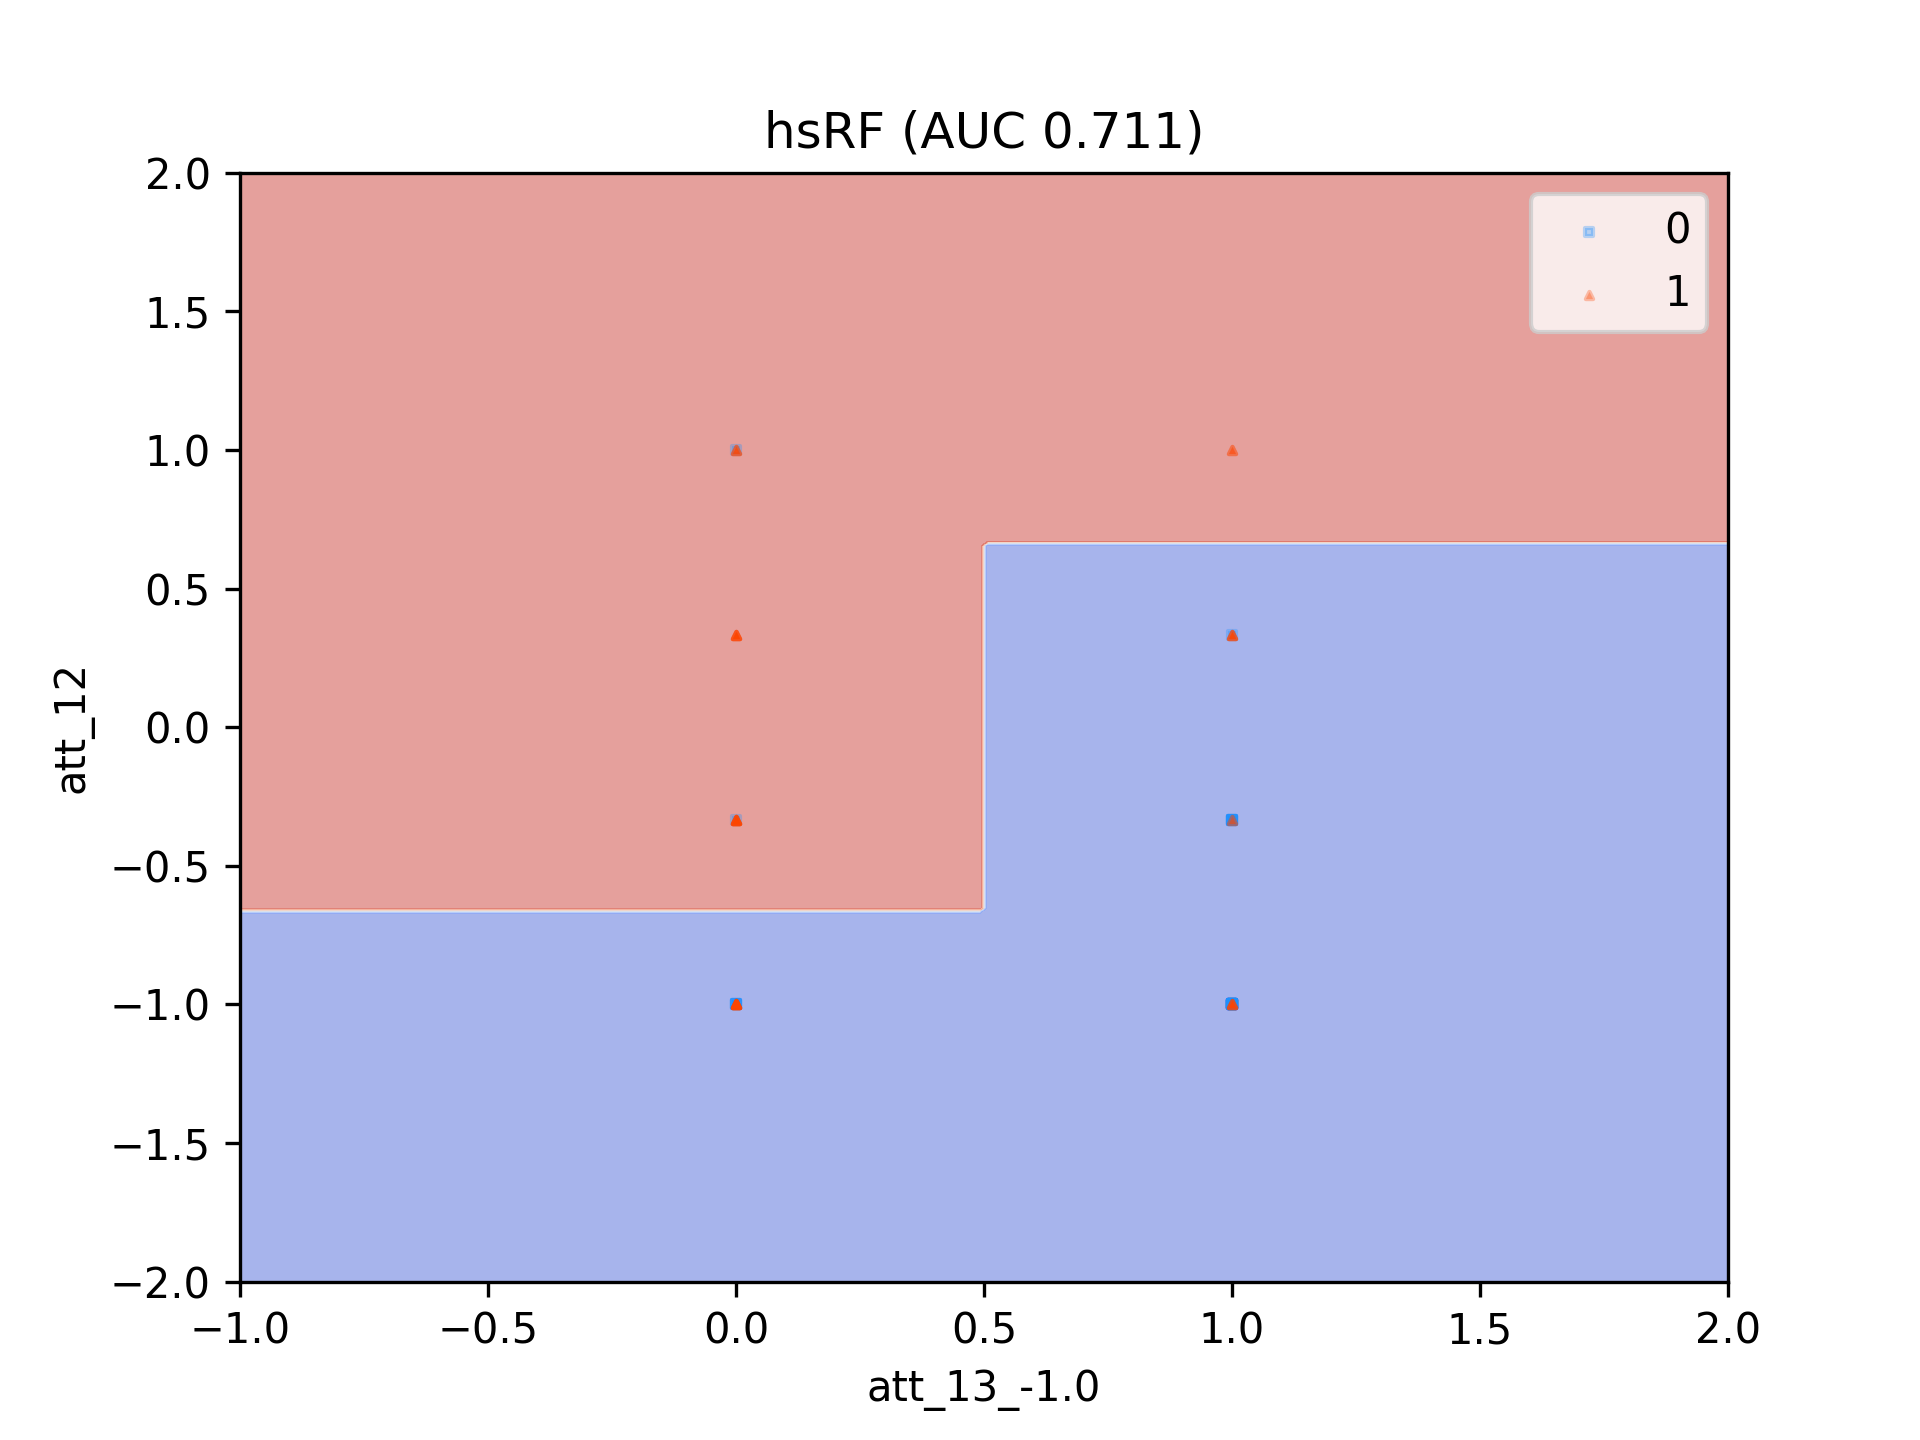
\includegraphics[width=\textwidth]{images/appendix4/boundaries/heart_hsRF_reproduced.png}
        \caption{Heart hsRF \\ (AUC 0.711)}
    \end{subfigure}
    
    \begin{subfigure}[b]{0.45\textwidth}
        \centering
        \includegraphics[width=\textwidth]{images/appendix4/boundaries/breast_cancer_RF_reproduced.png}
        \caption{Breast cancer RF \\ (AUC 0.505)}
    \end{subfigure}
    \begin{subfigure}[b]{0.45\textwidth}
        \centering
        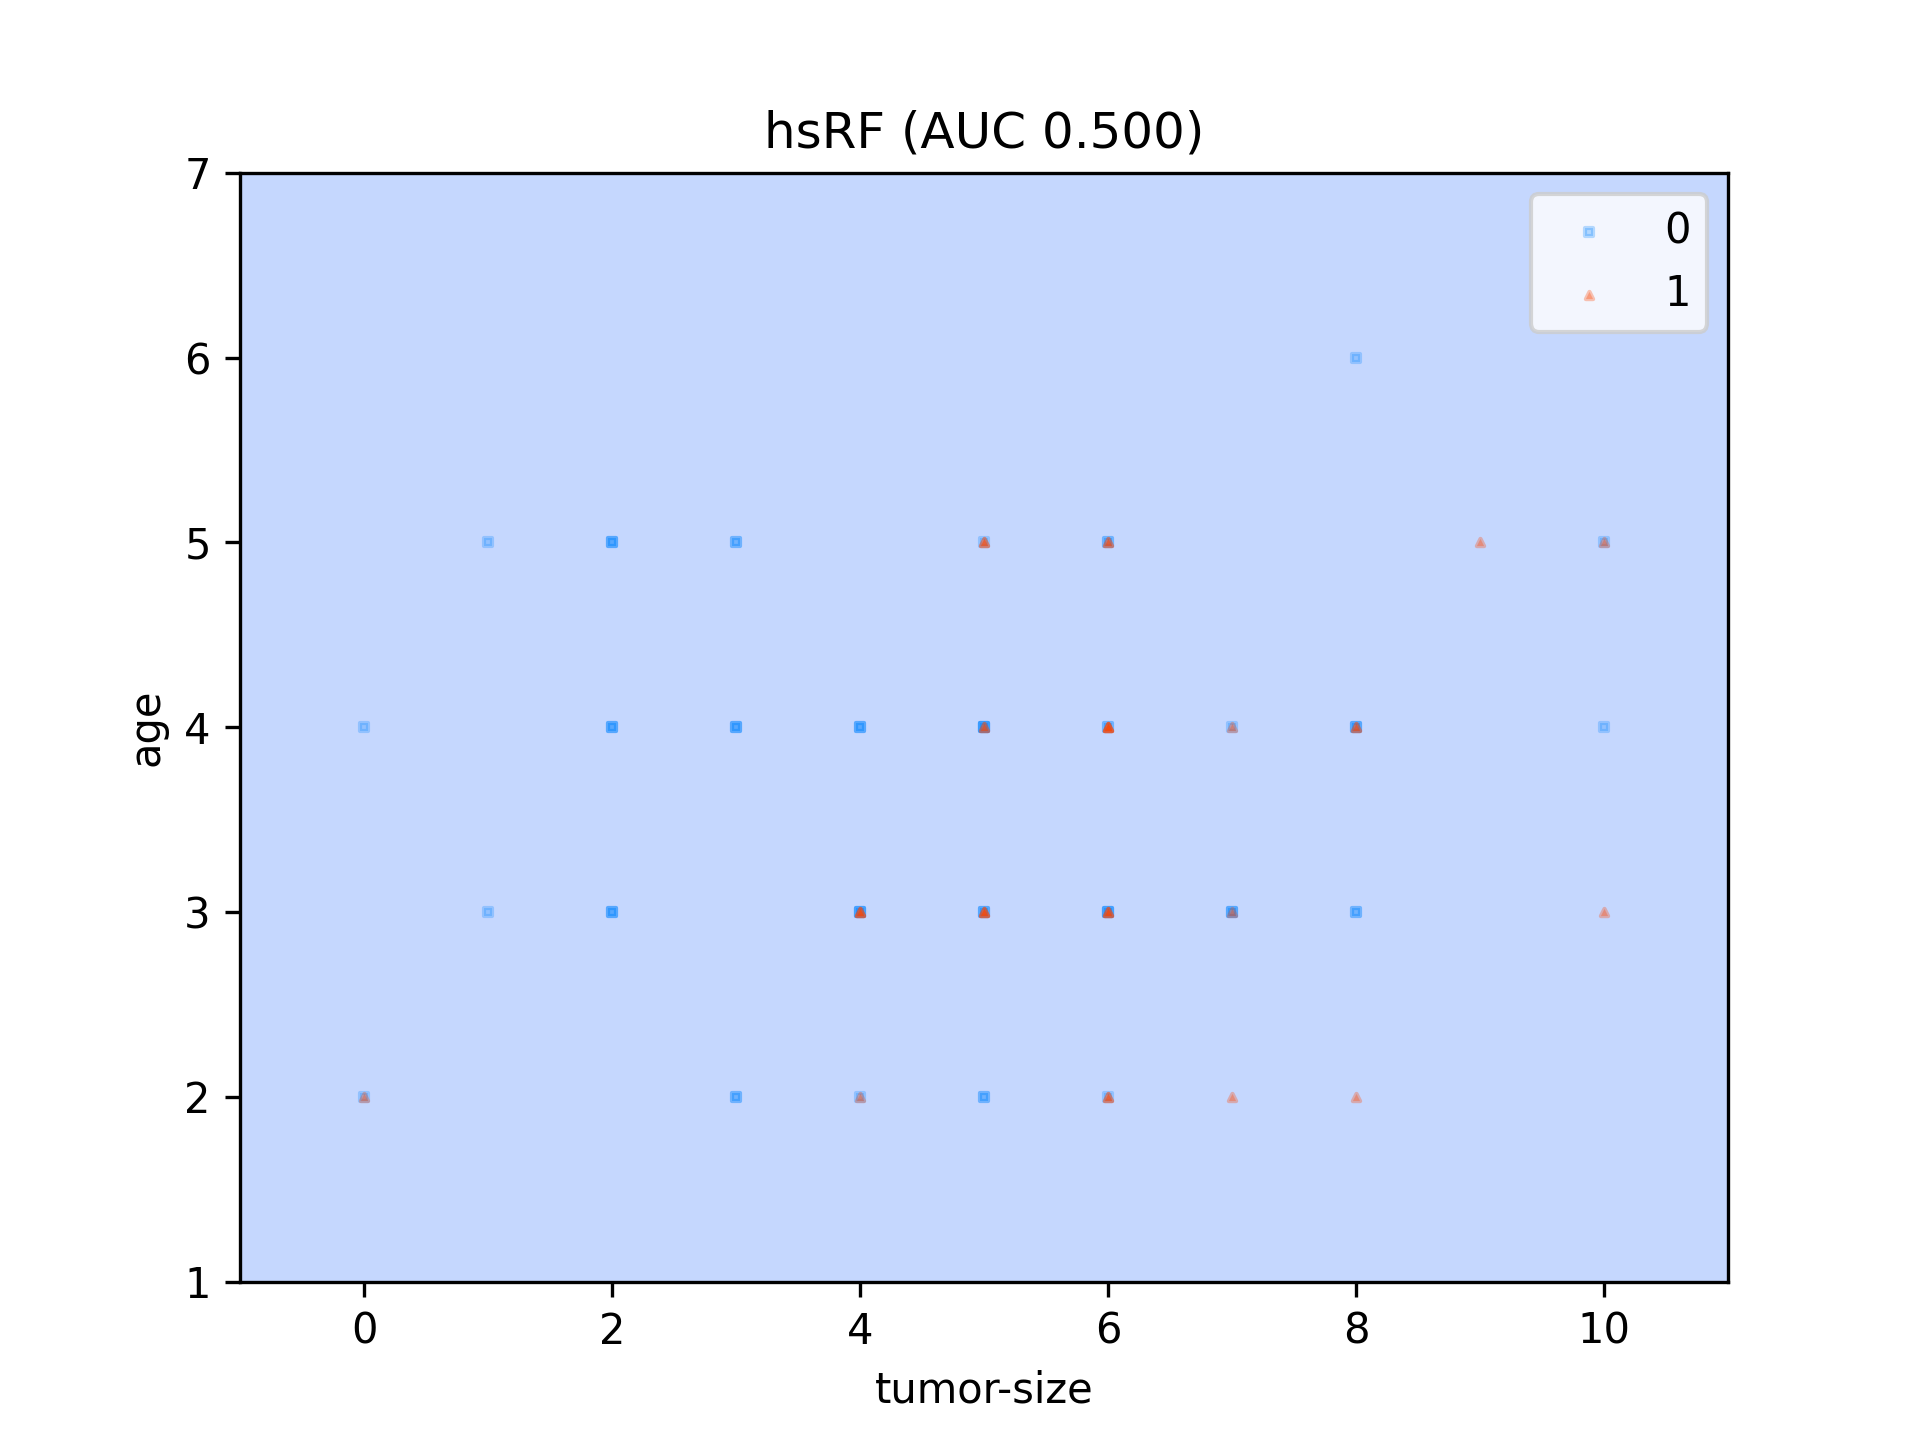
\includegraphics[width=\textwidth]{images/appendix4/boundaries/breast_cancer_hsRF_reproduced.png}
        \caption{Breast cancer hsRF \\ (AUC 0.500)}
    \end{subfigure}
    
    \begin{subfigure}[b]{0.45\textwidth}
        \centering
        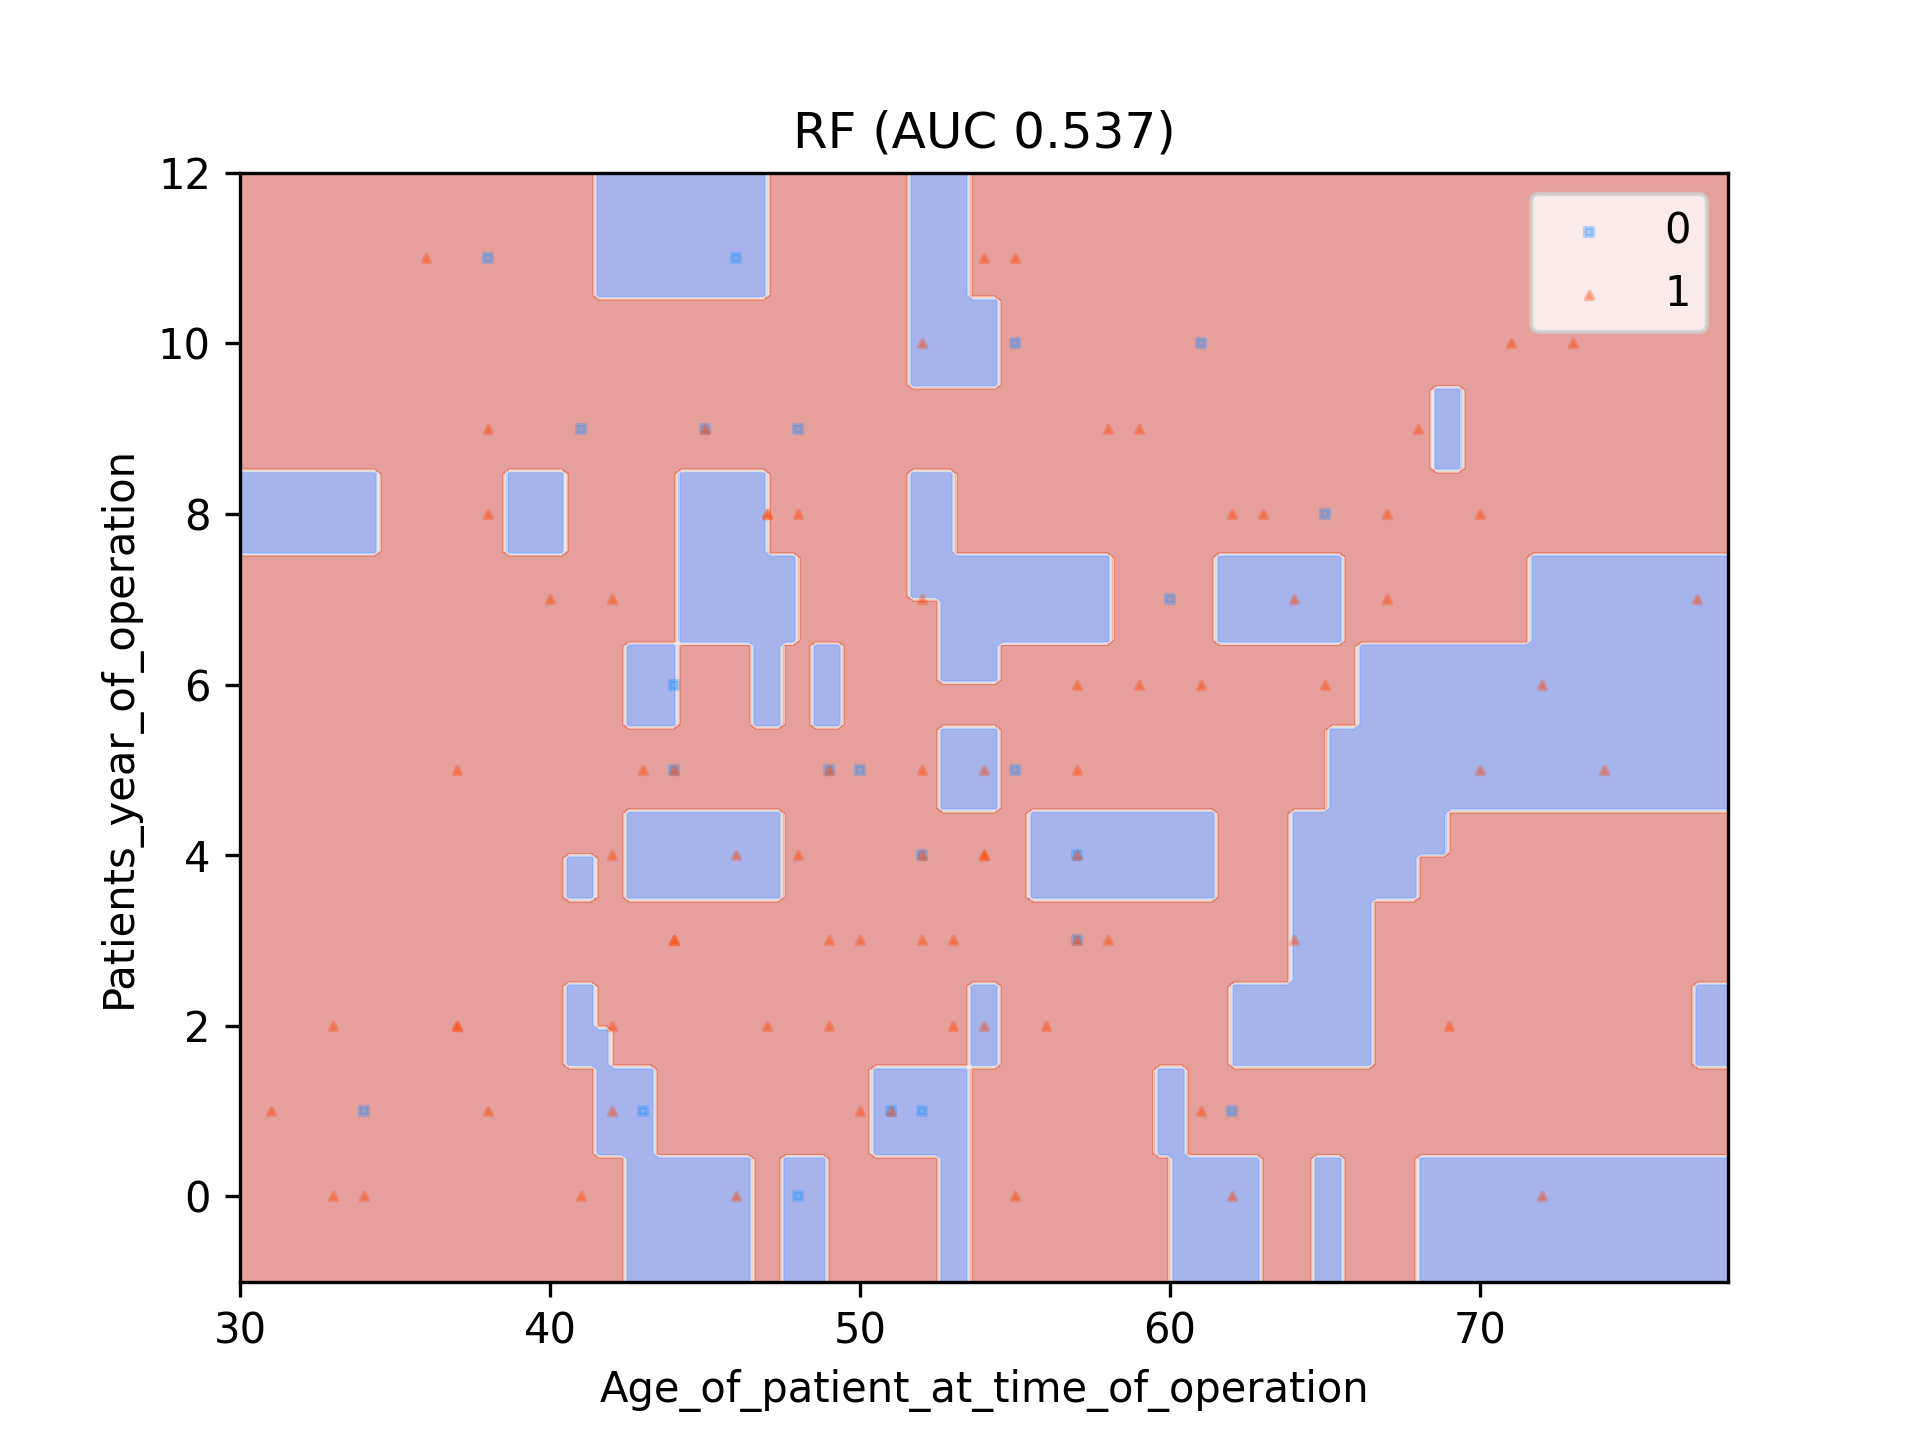
\includegraphics[width=\textwidth]{images/appendix4/boundaries/haberman_RF_reproduced.png}
        \caption{Haberman RF \\ (AUC 0.537)}
    \end{subfigure}
    \begin{subfigure}[b]{0.45\textwidth}
        \centering
        \includegraphics[width=\textwidth]{images/appendix4/boundaries/haberman_hsRF_reproduced.png}
        \caption{Haberman hsRF \\ (AUC 0.464)}
    \end{subfigure}
    
    \begin{subfigure}[b]{0.45\textwidth}
        \centering
        \includegraphics[width=\textwidth]{images/appendix4/boundaries/ionosphere_RF_reproduced.png}
        \caption{Ionosphere RF \\ (AUC 0.869)}
    \end{subfigure}
    \begin{subfigure}[b]{0.45\textwidth}
        \centering
        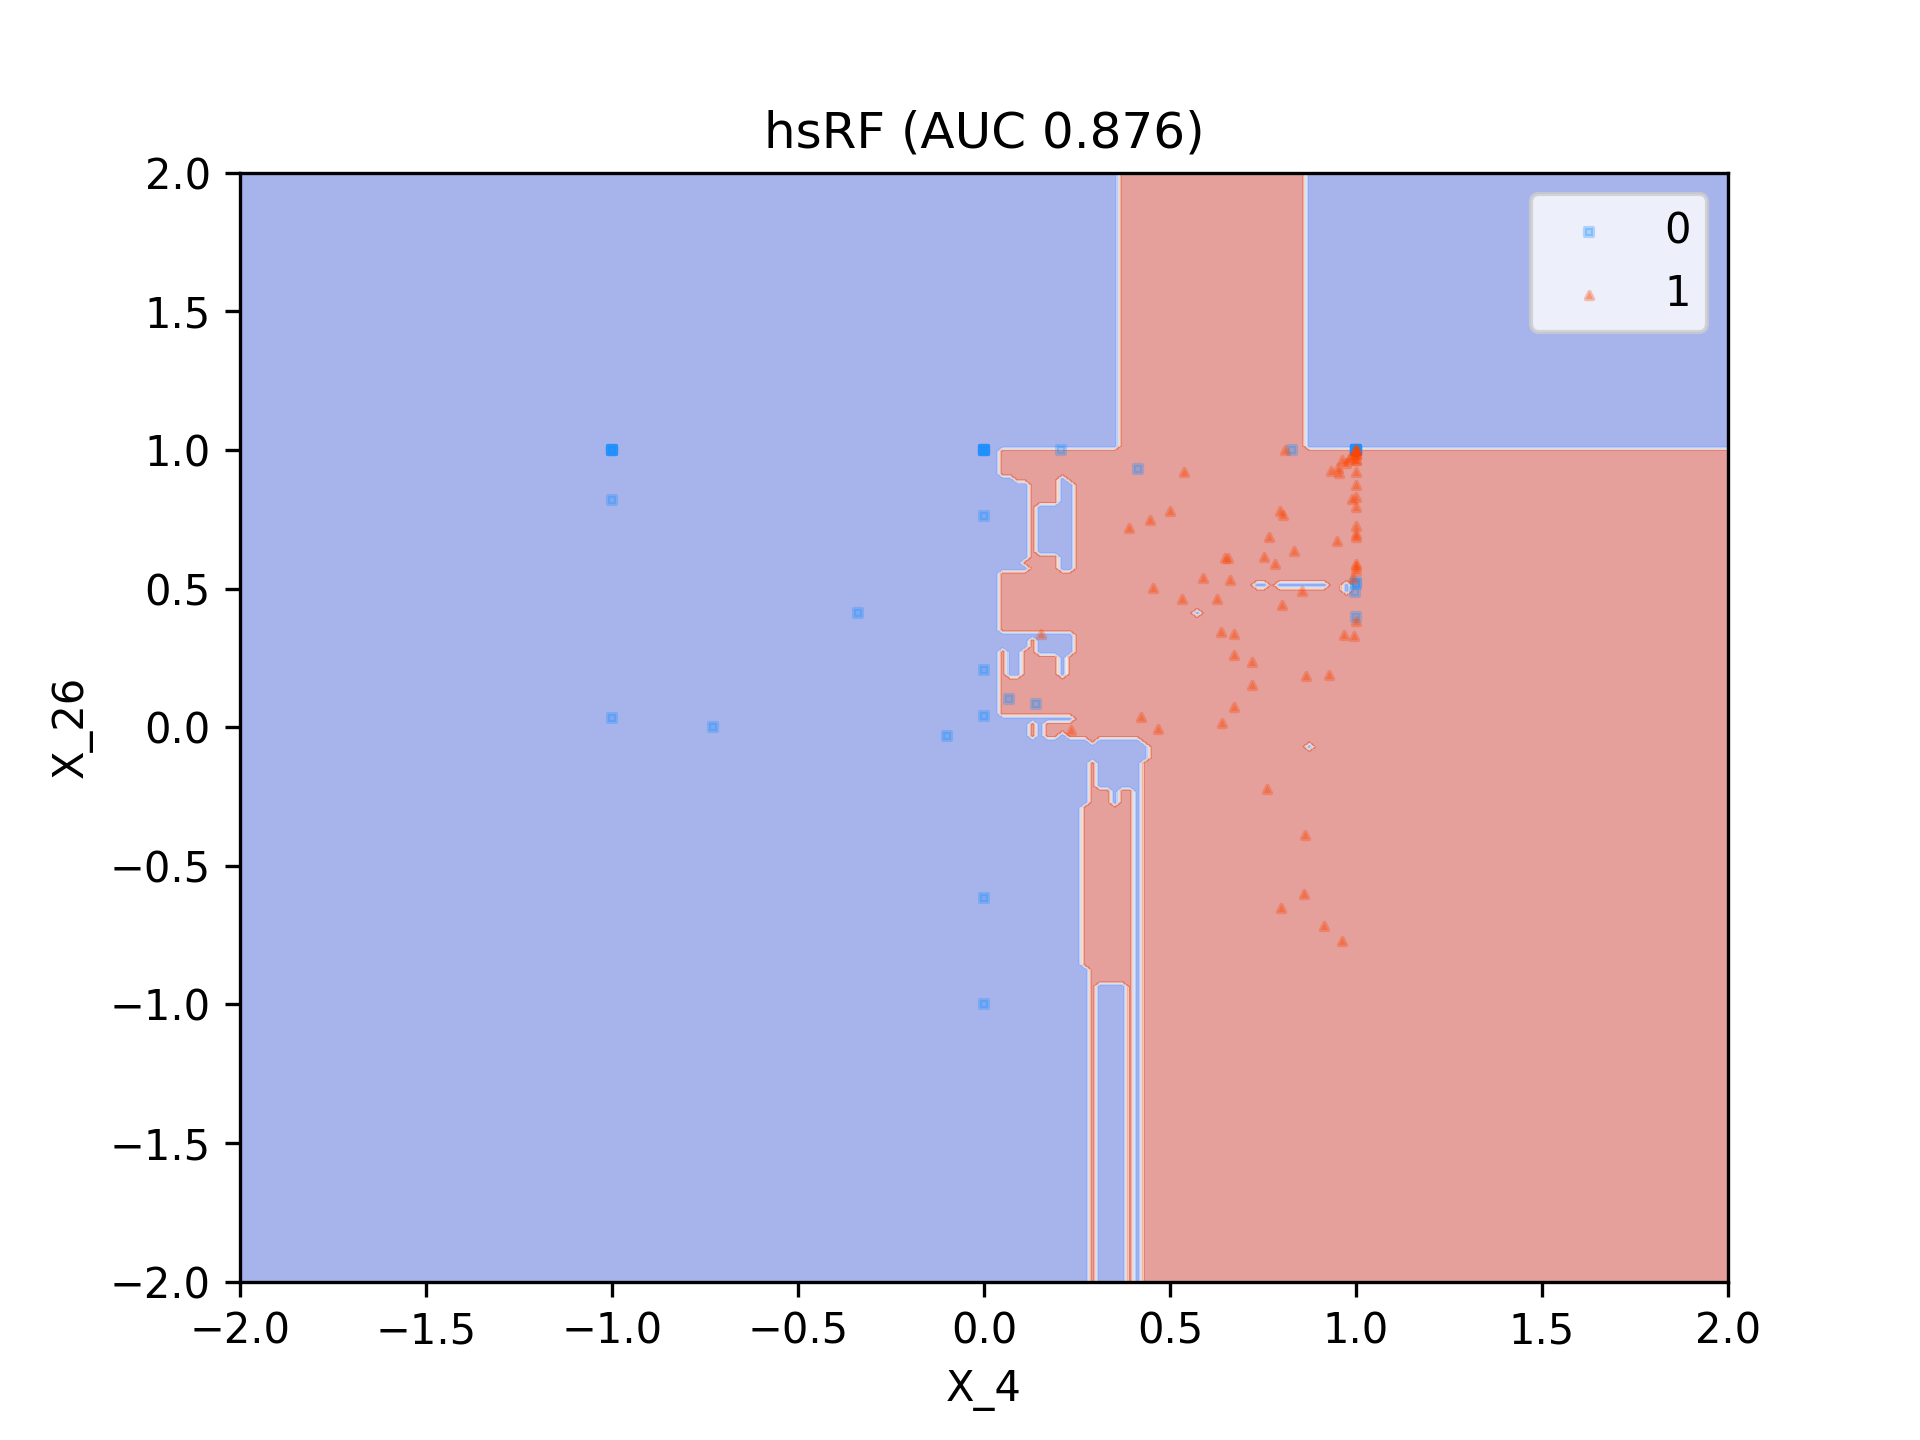
\includegraphics[width=\textwidth]{images/appendix4/boundaries/ionosphere_hsRF_reproduced.png}
        \caption{Ionosphere hsRF \\ (AUC 0.876)}
    \end{subfigure}
    \caption{Comparison of decision boundaries for the first four classification data sets as learned by RF before and after applying HS.}
    \label{fig:apx4-boundary1}
\end{figure}

\begin{figure}[hbt]
    \centering
    \begin{subfigure}[b]{0.45\textwidth}
        \centering
        \includegraphics[width=\textwidth]{images/appendix4/boundaries/diabetes_RF_reproduced.png}
        \caption{Diabetes RF \\ (AUC 0.700)}
    \end{subfigure}
    \begin{subfigure}[b]{0.45\textwidth}
        \centering
        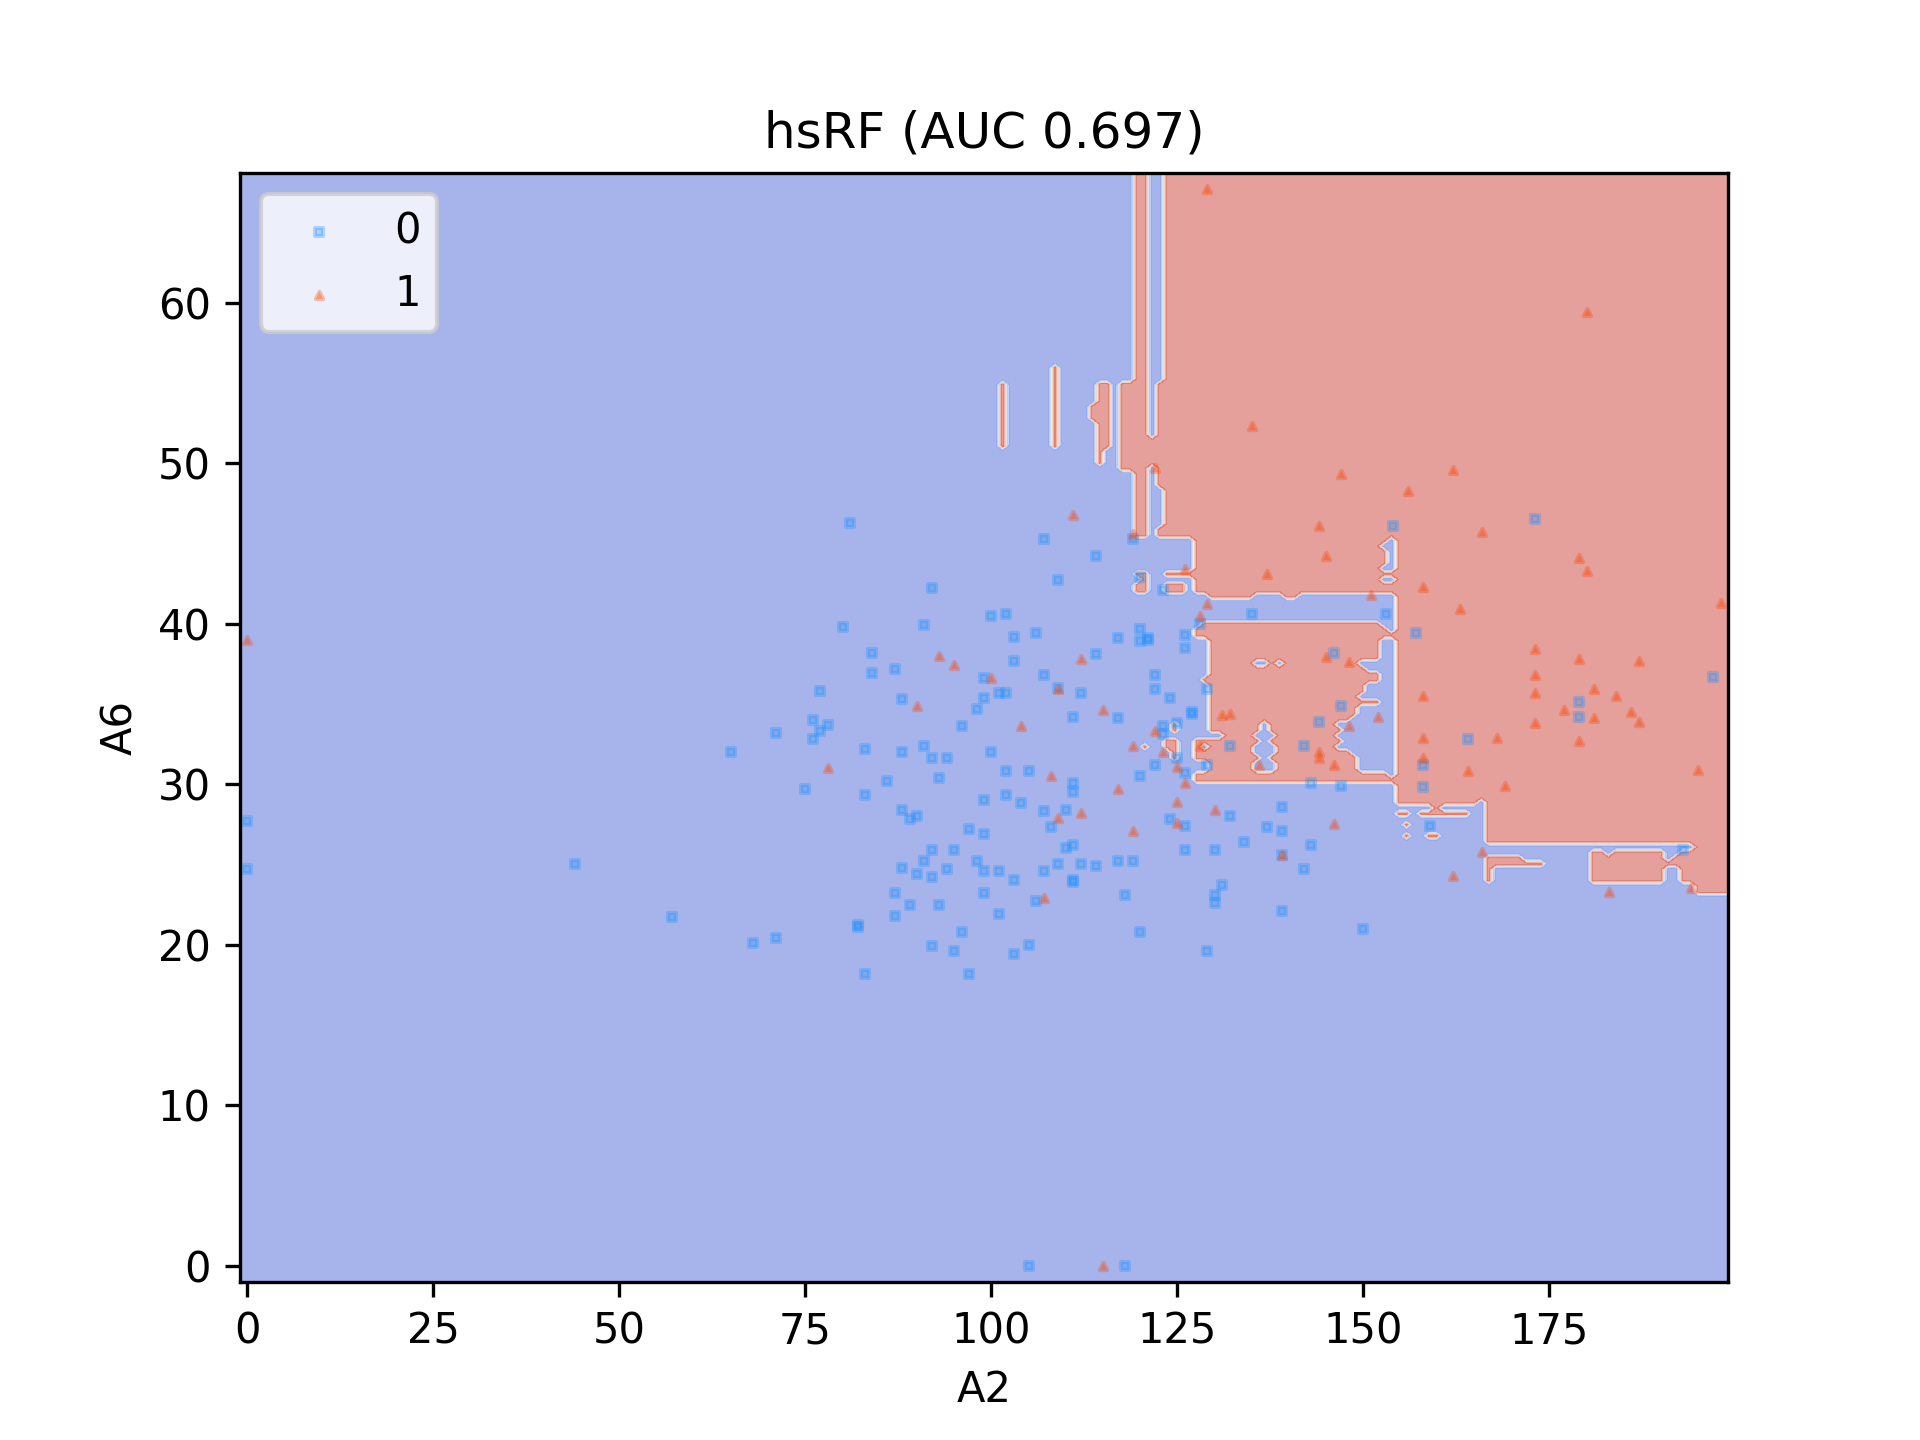
\includegraphics[width=\textwidth]{images/appendix4/boundaries/diabetes_hsRF_reproduced.png}
        \caption{Diabetes hsRF \\ (AUC 0.697)}
    \end{subfigure}
    
    \begin{subfigure}[b]{0.45\textwidth}
        \centering
        \includegraphics[width=\textwidth]{images/appendix4/boundaries/german_RF_reproduced.png}
        \caption{German credit RF \\ (AUC 0.594)}
    \end{subfigure}
    \begin{subfigure}[b]{0.45\textwidth}
        \centering
        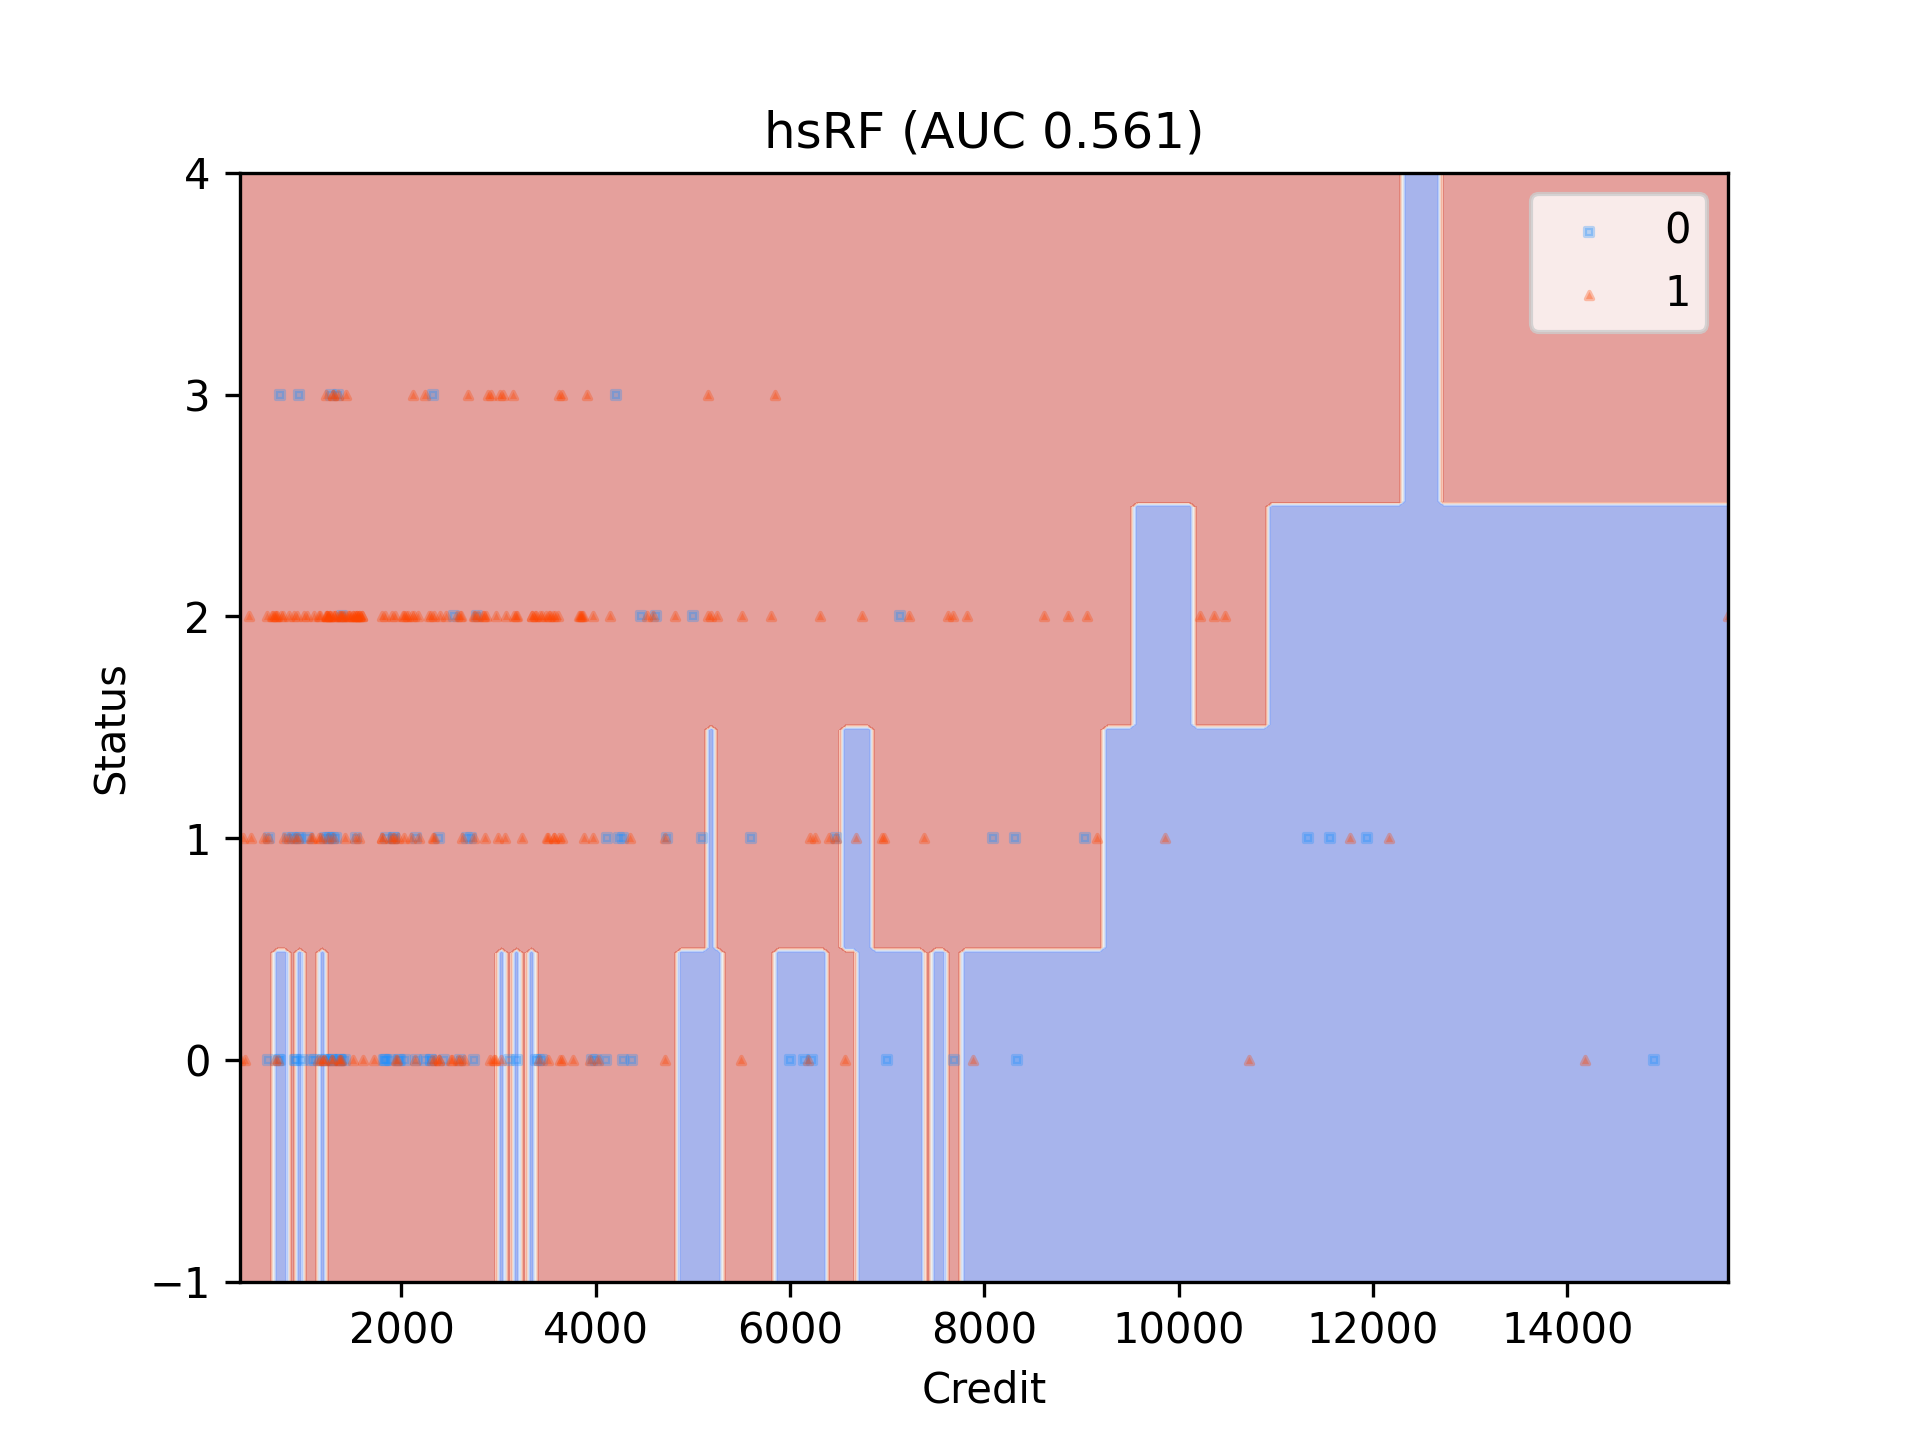
\includegraphics[width=\textwidth]{images/appendix4/boundaries/german_hsRF_reproduced.png}
        \caption{German credit hsRF \\ (AUC 0.561)}
    \end{subfigure}
    
    \begin{subfigure}[b]{0.45\textwidth}
        \centering
        \includegraphics[width=\textwidth]{images/appendix4/boundaries/juvenile_clean_RF_reproduced.png}
        \caption{Juvenile RF \\ (AUC 0.671)}
    \end{subfigure}
    \begin{subfigure}[b]{0.45\textwidth}
        \centering
        \includegraphics[width=\textwidth]{images/appendix4/boundaries/juvenile_clean_hsRF_reproduced.png}
        \caption{Juvenile hsRF \\ (AUC 0.671)}
    \end{subfigure}
    
    \begin{subfigure}[b]{0.45\textwidth}
        \centering
        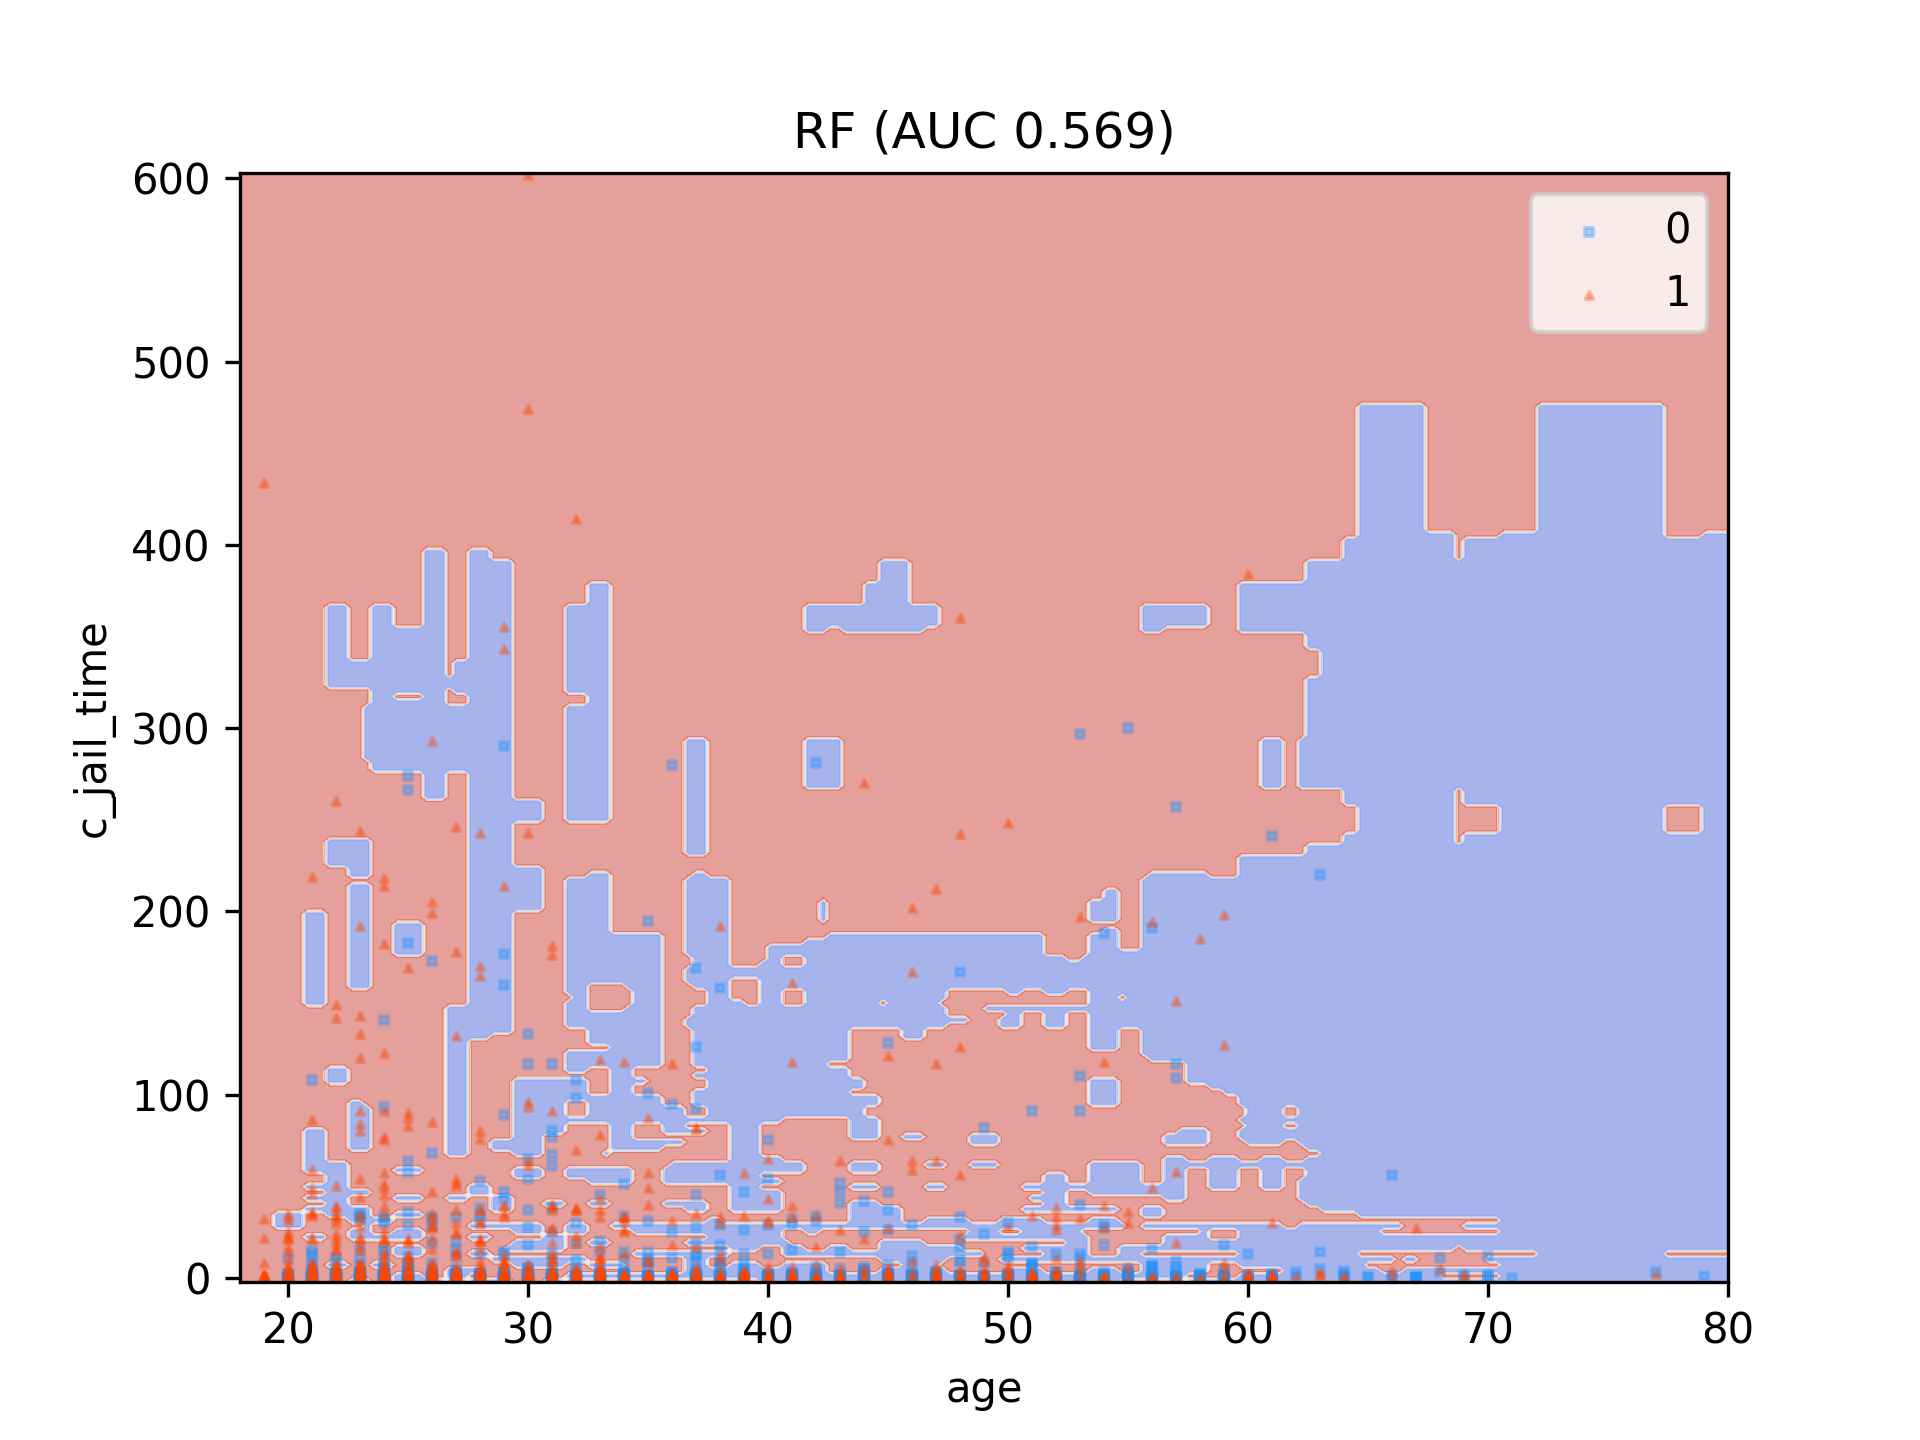
\includegraphics[width=\textwidth]{images/appendix4/boundaries/compas_two_year_clean_RF_reproduced.png}
        \caption{Recidivism RF \\ (AUC 0.569)}
    \end{subfigure}
    \begin{subfigure}[b]{0.45\textwidth}
        \centering
        \includegraphics[width=\textwidth]{images/appendix4/boundaries/compas_two_year_clean_hsRF_reproduced.png}
        \caption{Recidivism hsRF \\ (AUC 0.606)}
    \end{subfigure}
    \caption{Comparison of decision boundaries for the last four classification data sets as learned by RF before and after applying HS.}
    \label{fig:apx4-boundary2}
\end{figure}

\subsection{SHAP plots and variability}
\label{appendix:claim4-shap}

In this section we investigate how HS influences the SHAP value plots and their variability for RF with and without HS. The experiment was done by witholding 50 data points from a classification problem, build a RF with 2/3 of the remaining data, and evaluate SHAP values for each held out sample. This was repeated 100 times. We then averaged the variance for each feature across all held out samples.

Value plots for classification data sets are on Fig.~\ref{fig:apx4-sval1} and Fig.~\ref{fig:apx4-sval2}. We can see that after applying HS the explanations for each feature have tighter clusters, and explanations are less noisy.

\begin{figure}[hbt]
    \centering
    \begin{subfigure}[b]{0.90\textwidth}
        \centering
        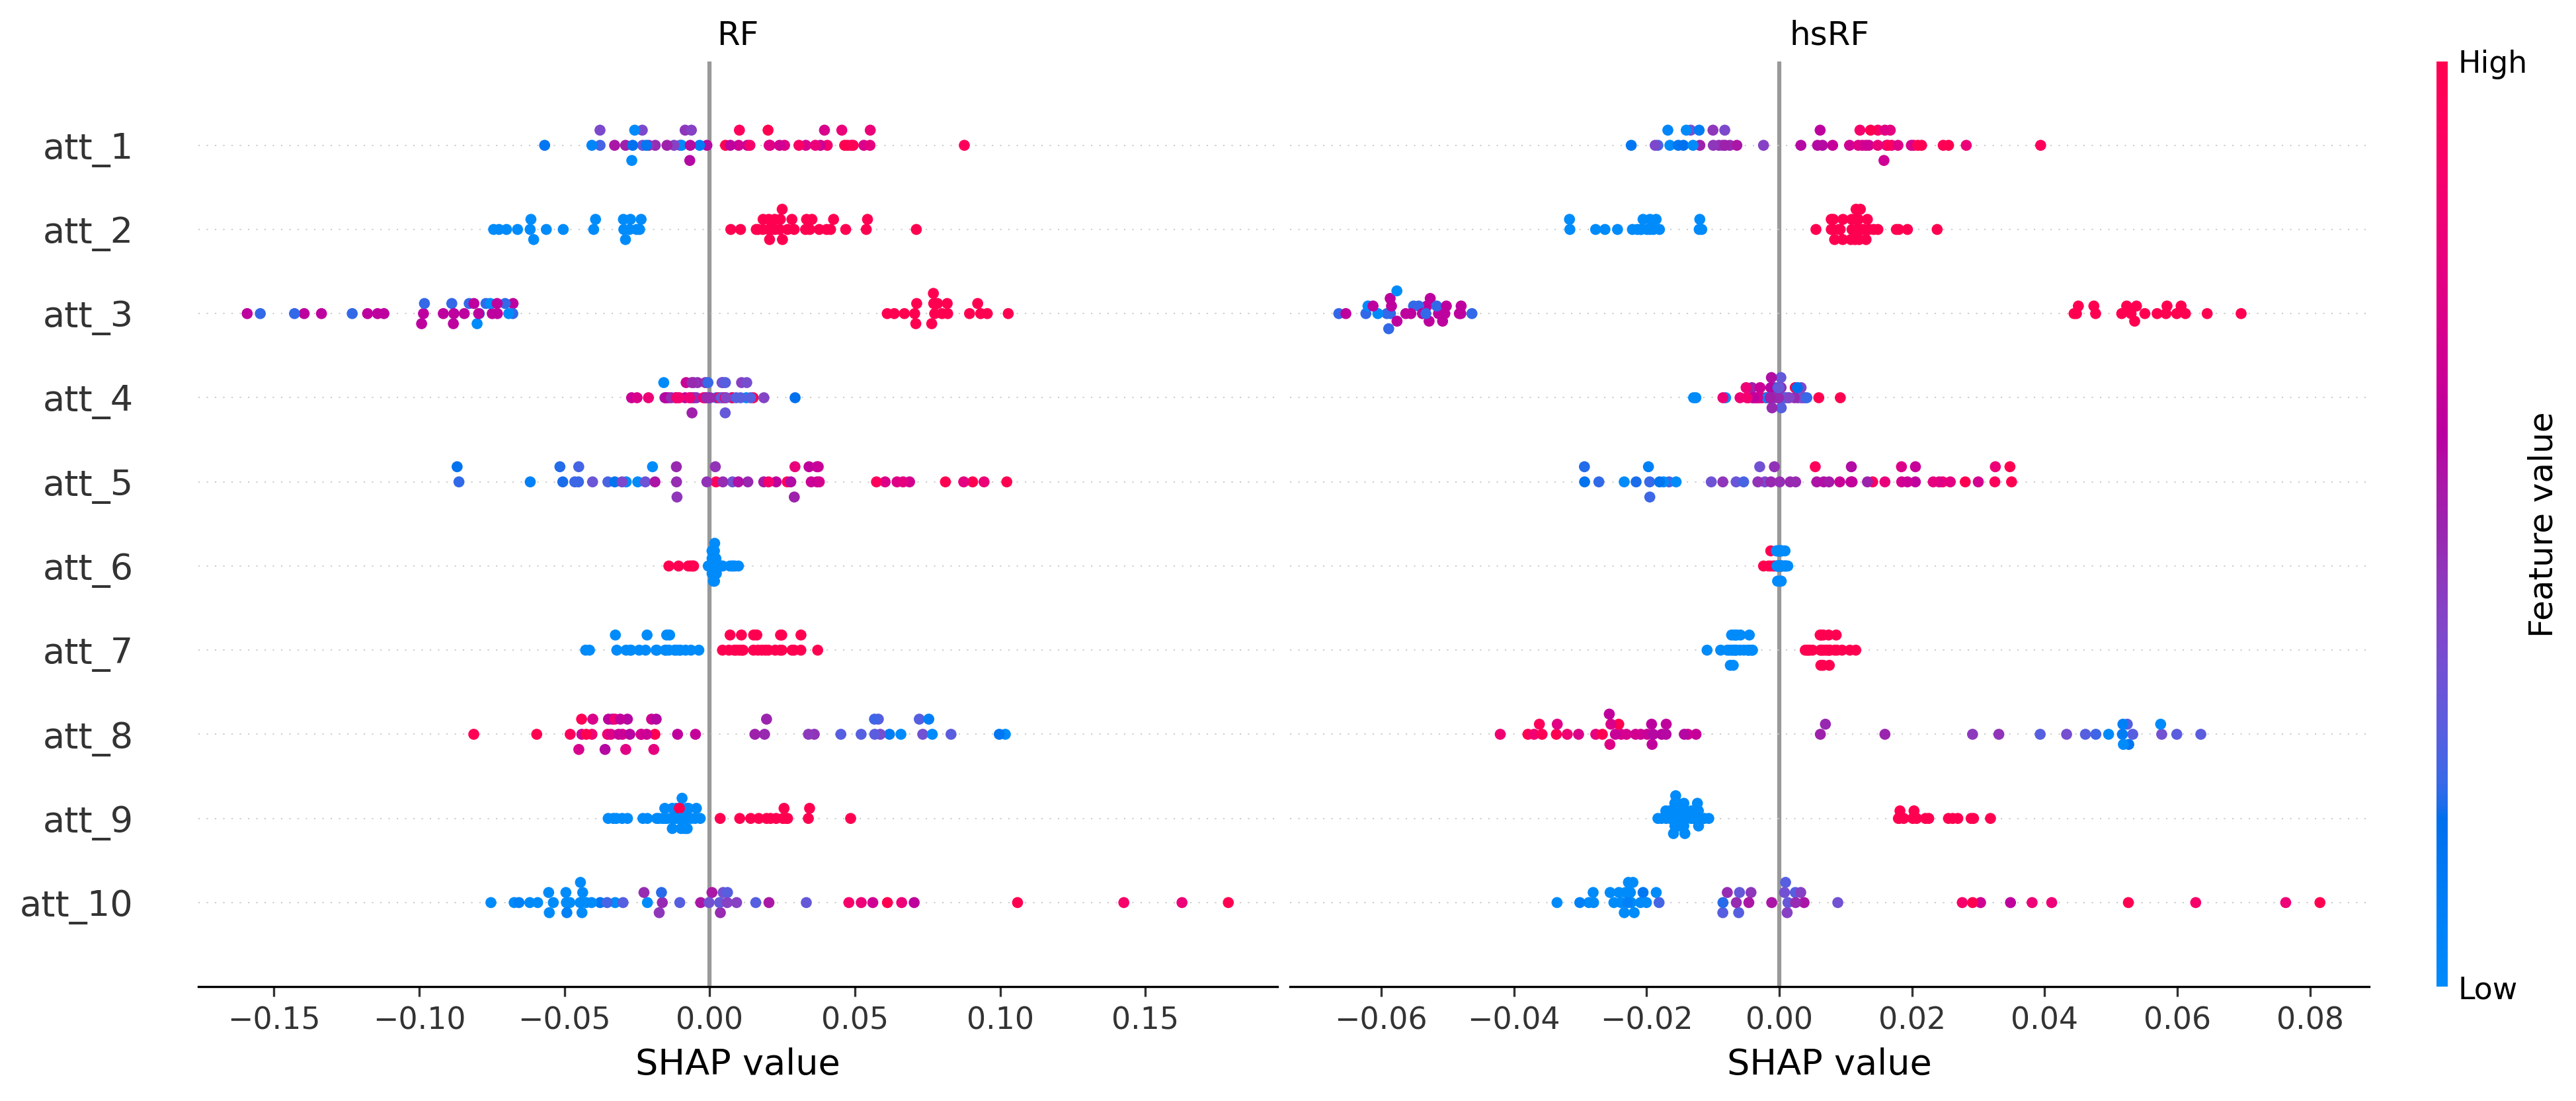
\includegraphics[width=\textwidth]{images/appendix4/SHAP_interpretation/heart.png}
        \caption{Heart}
    \end{subfigure}
    
    \begin{subfigure}[b]{0.90\textwidth}
        \centering
        \includegraphics[width=\textwidth]{images/appendix4/SHAP_interpretation/breast_cancer.png}
        \caption{Breast cancer}
    \end{subfigure}
    
    \begin{subfigure}[b]{0.90\textwidth}
        \centering
        \includegraphics[width=\textwidth]{images/appendix4/SHAP_interpretation/haberman.png}
        \caption{Haberman}
    \end{subfigure}
    
    \begin{subfigure}[b]{0.90\textwidth}
        \centering
        \includegraphics[width=\textwidth]{images/appendix4/SHAP_interpretation/ionosphere.png}
        \caption{Ionosphere}
    \end{subfigure}
    \caption{Comparison of SHAP value plots for the first four classification data sets before and after applying HS.}
    \label{fig:apx4-sval1}
\end{figure}

\begin{figure}[hbt]
    \centering
    \begin{subfigure}[b]{0.80\textwidth}
        \centering
        \includegraphics[width=\textwidth]{images/appendix4/SHAP_interpretation/diabetes.png}
        \caption{Diabetes RF}
    \end{subfigure}
    
    \begin{subfigure}[b]{0.80\textwidth}
        \centering
        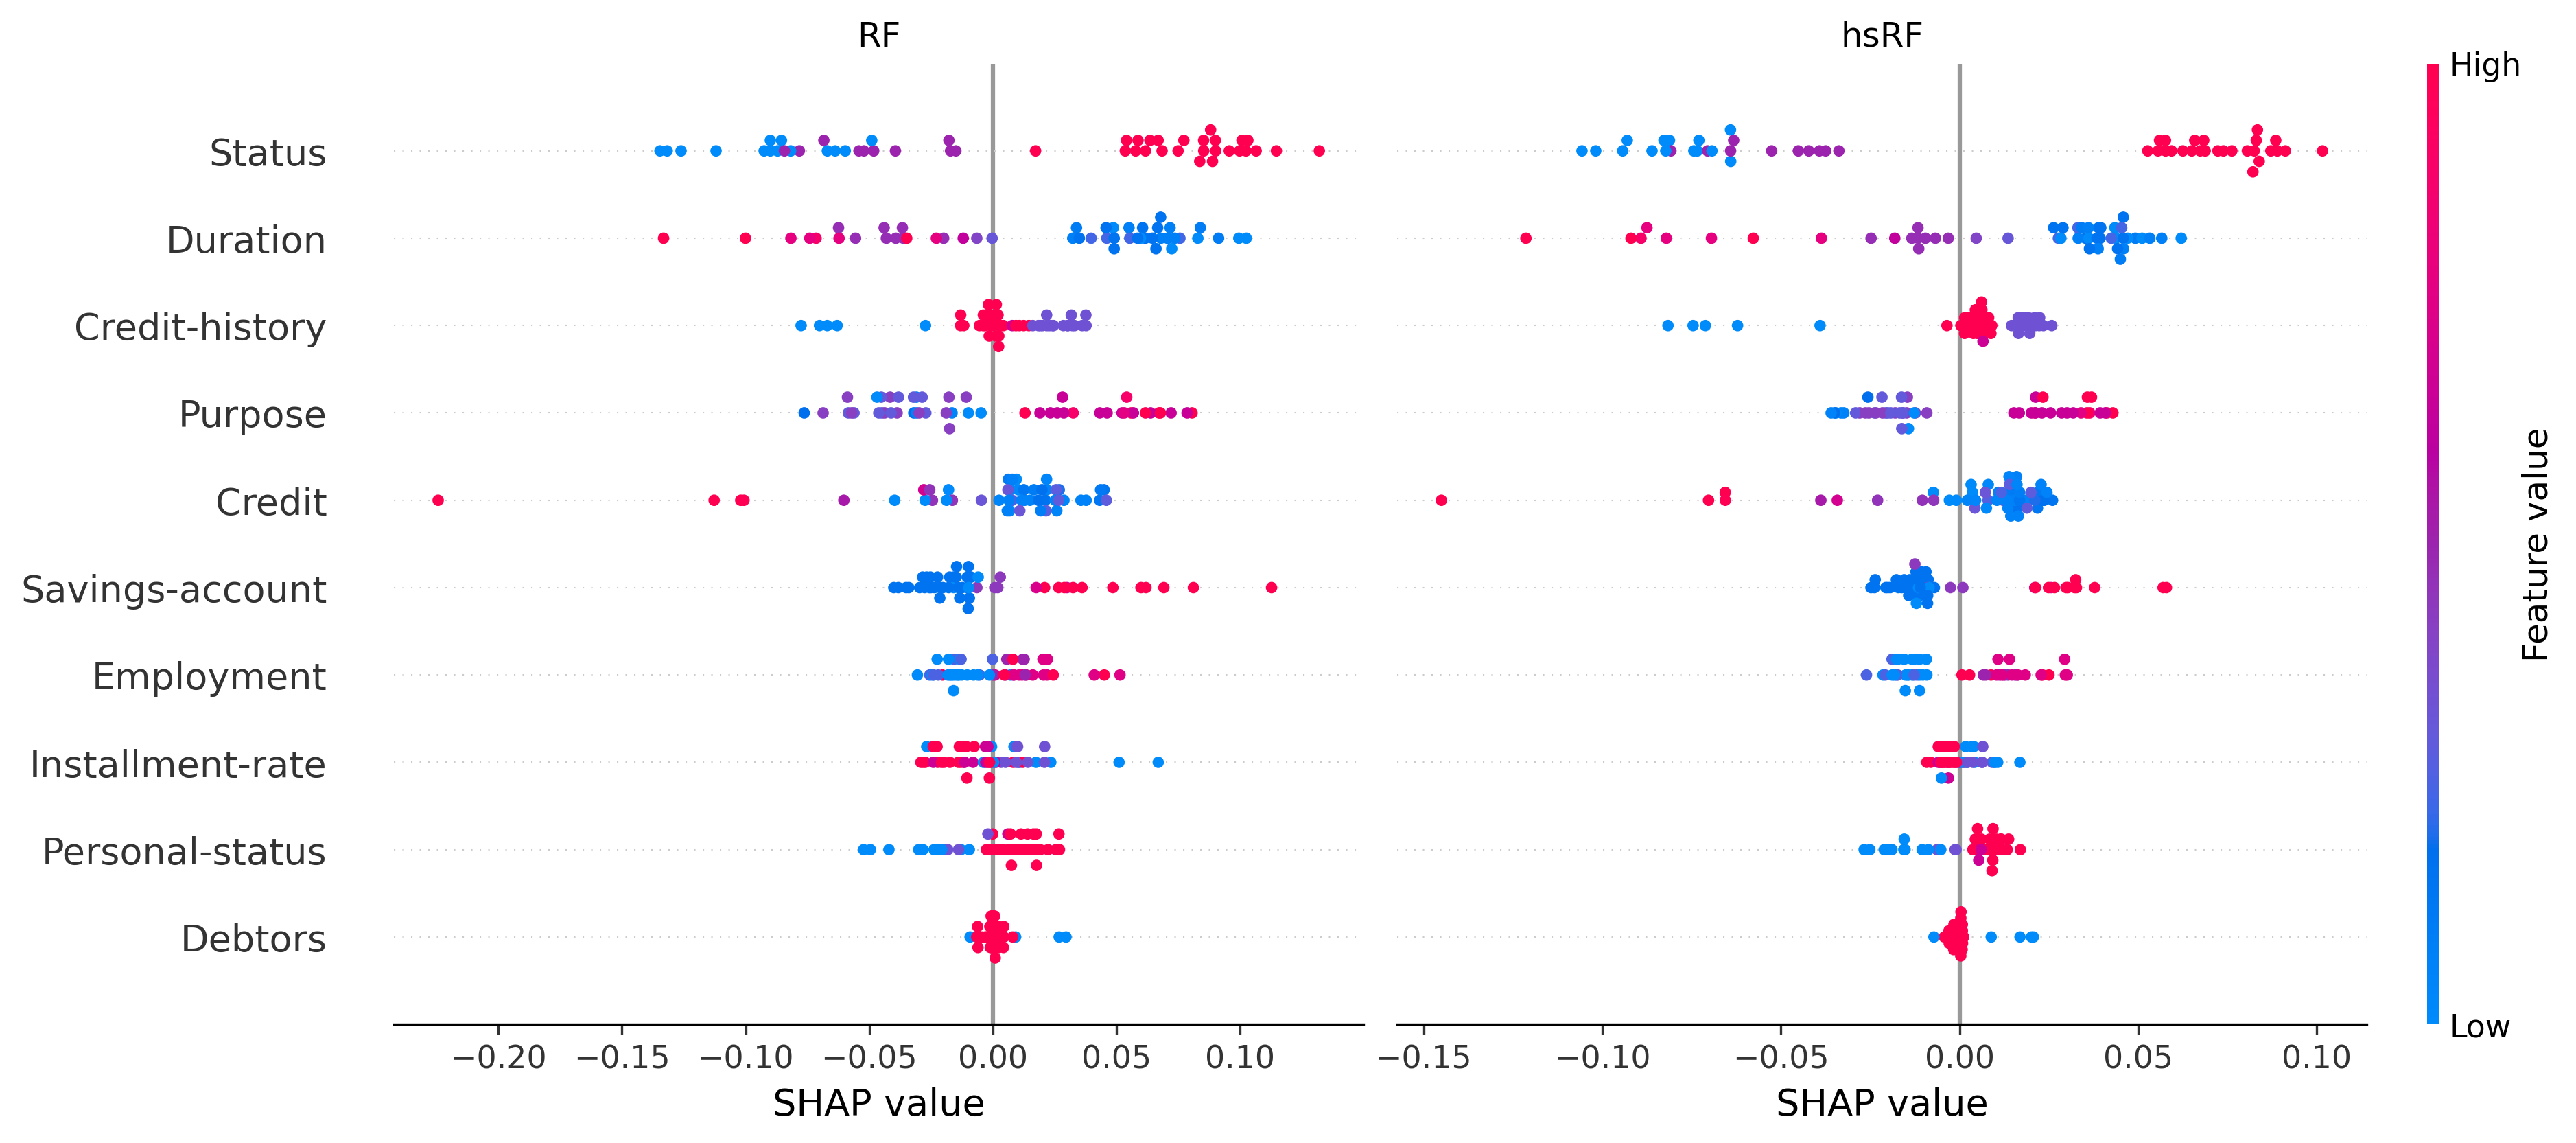
\includegraphics[width=\textwidth]{images/appendix4/SHAP_interpretation/german.png}
        \caption{German credit}
    \end{subfigure}
    
    \begin{subfigure}[b]{0.80\textwidth}
        \centering
        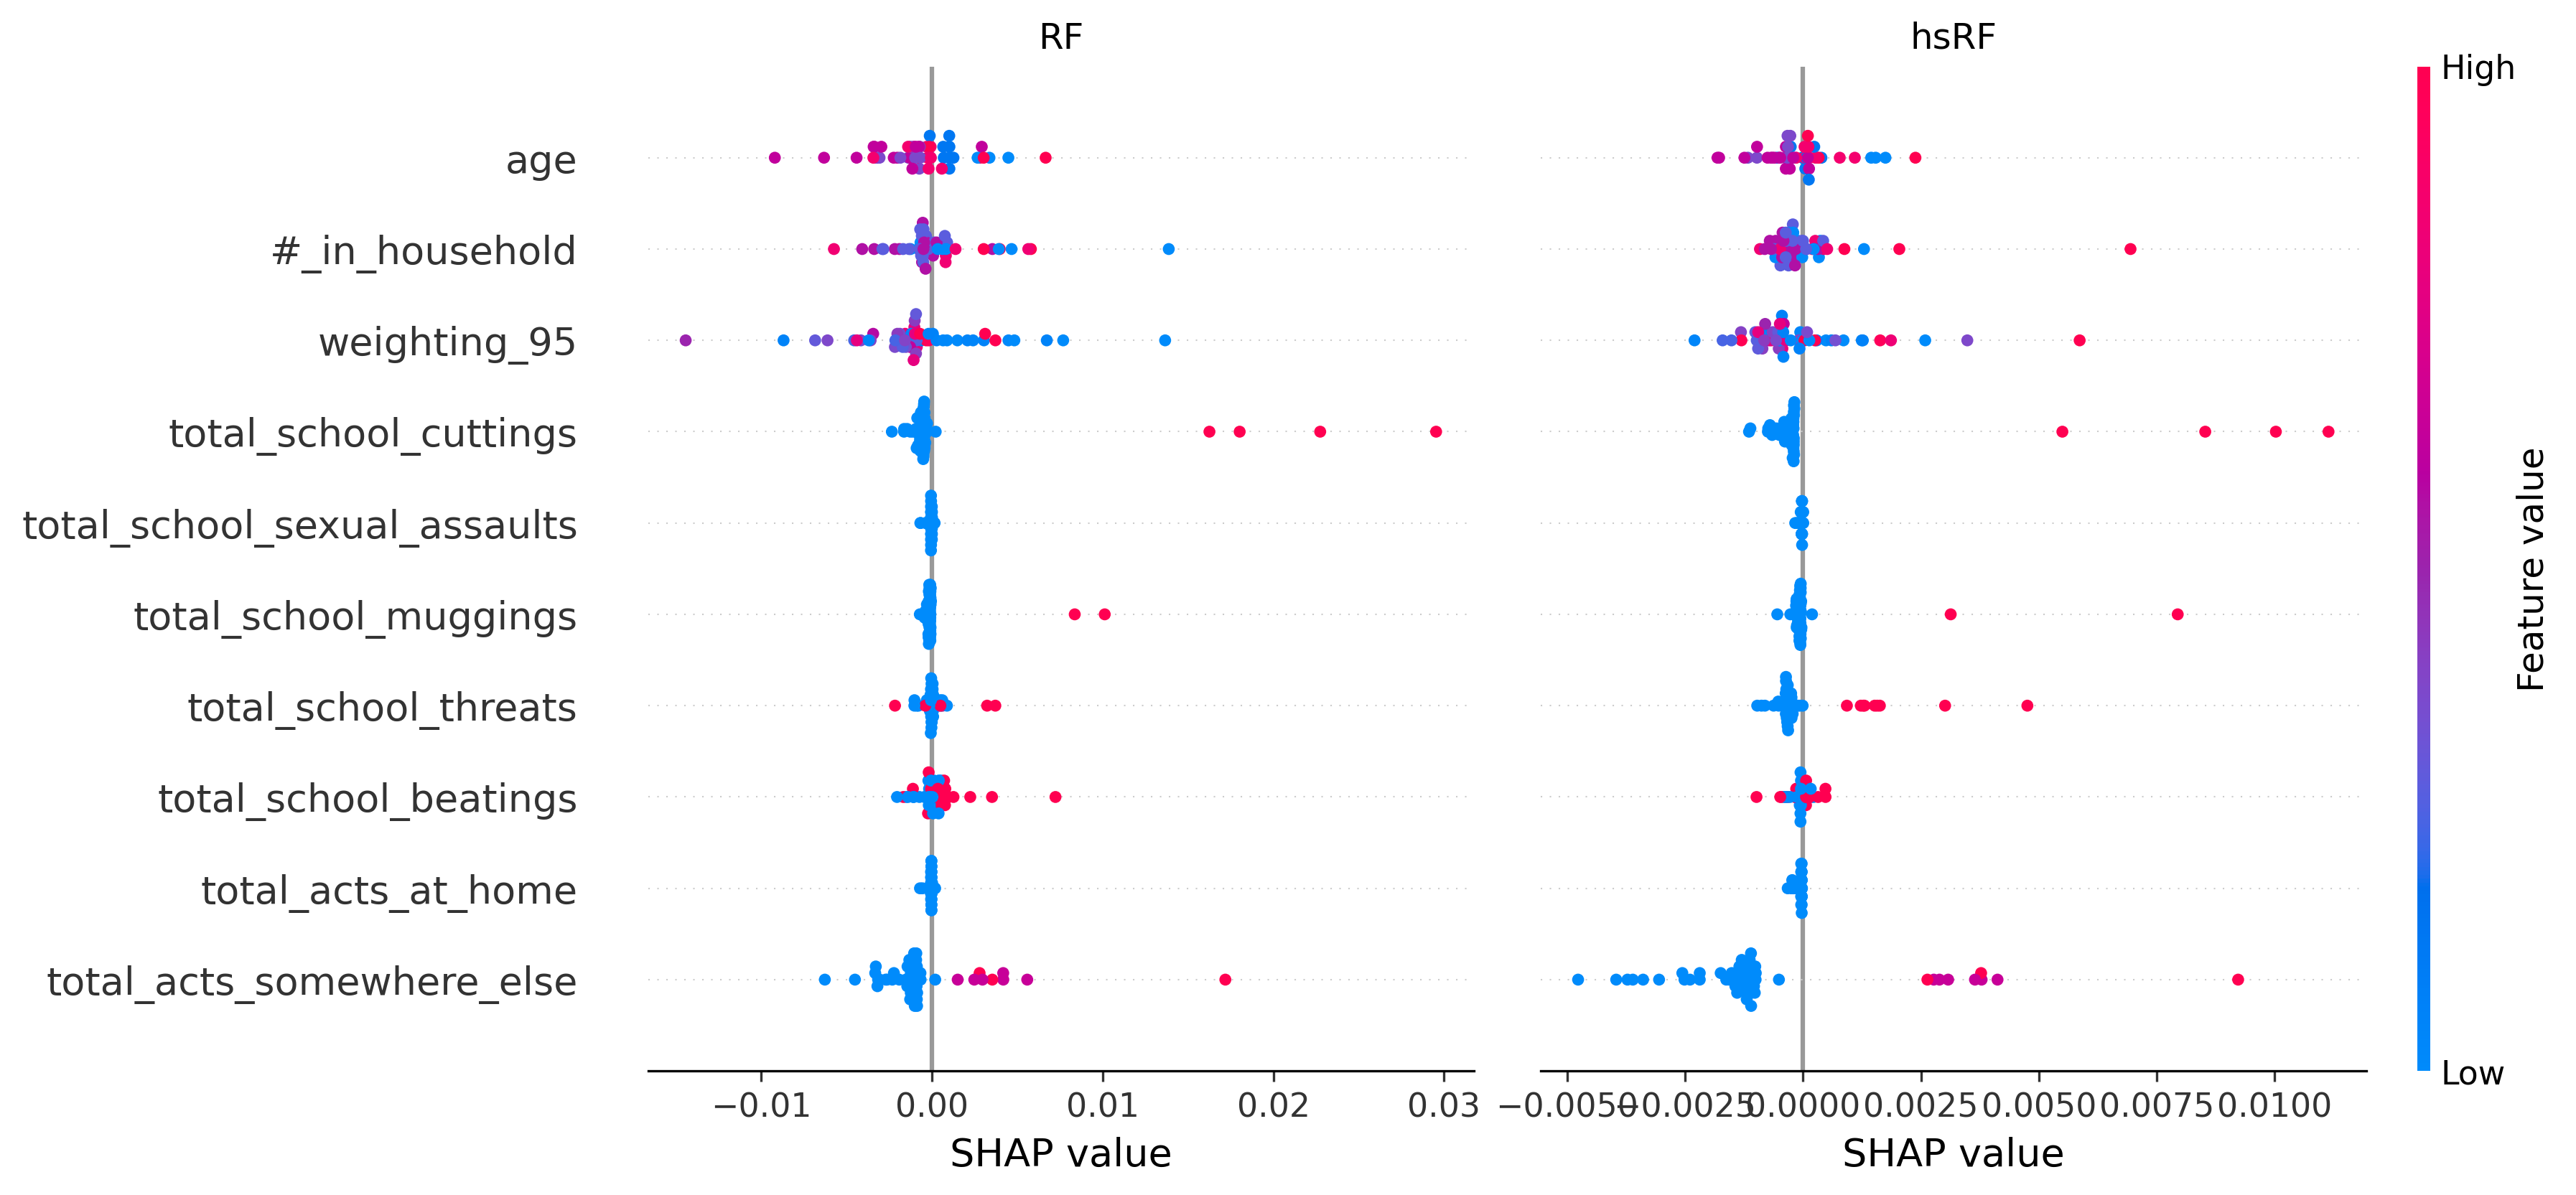
\includegraphics[width=\textwidth]{images/appendix4/SHAP_interpretation/juvenile_clean.png}
        \caption{Juvenile}
    \end{subfigure}
    
    \begin{subfigure}[b]{0.80\textwidth}
        \centering
        \includegraphics[width=\textwidth]{images/appendix4/SHAP_interpretation/compas_two_year_clean.png}
        \caption{Recidivism}
    \end{subfigure}
    \caption{Comparison of SHAP value plots for the last four classification data sets before and after applying HS.}
    \label{fig:apx4-sval2}
\end{figure}

We showed that HS clusters the explanations together, which means it reduces the explanation variance. The comparison of the variability of SHAP interpretations for classification data sets can be seen on Fig.~\ref{fig:apx4-svar1} and Fig.~\ref{fig:apx4-svar2}.

\begin{figure}[hbt]
    \centering
    \begin{subfigure}[t]{0.45\textwidth}
        \vskip 0pt
        \centering
        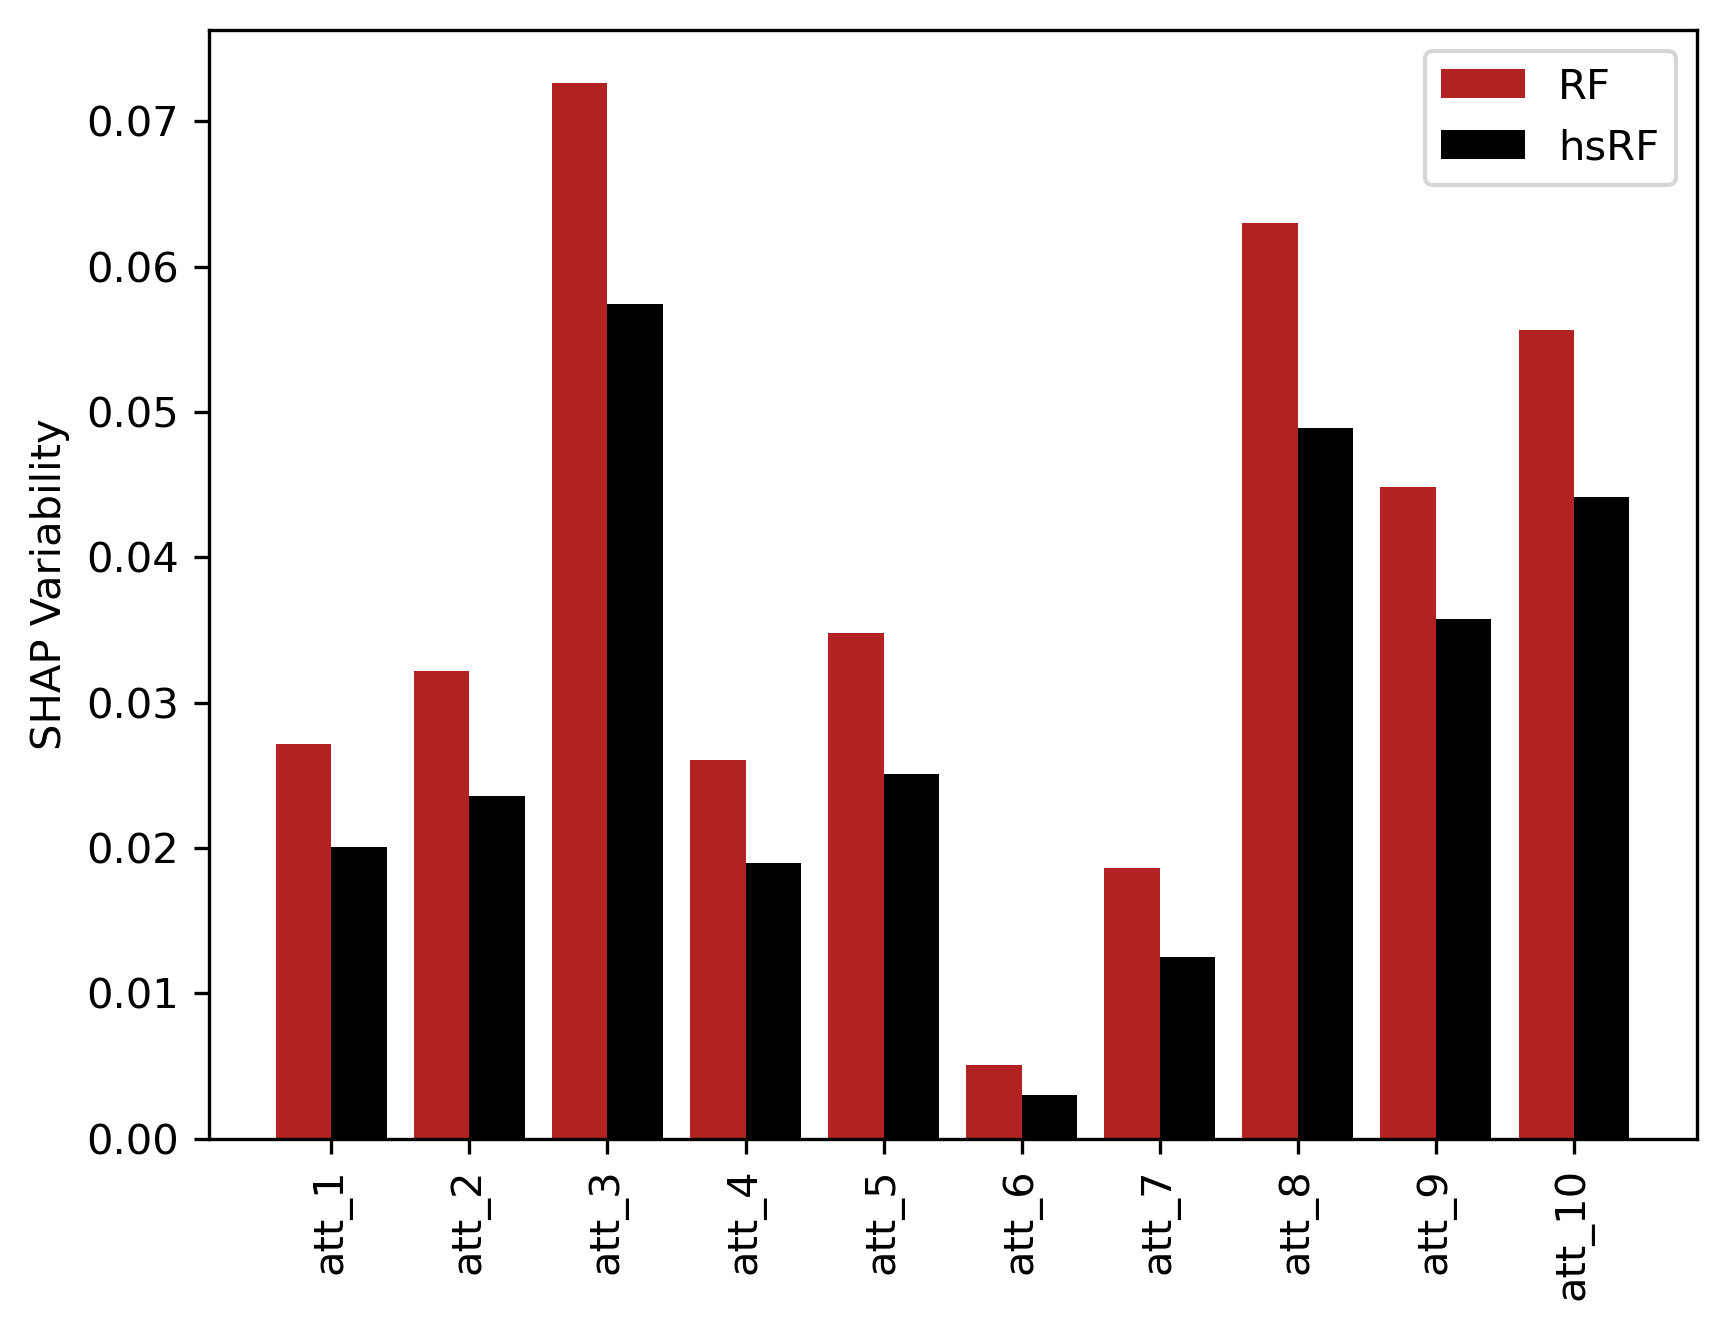
\includegraphics[width=\textwidth]{images/appendix4/SHAP_variability/heart.png}
        \caption{Heart}
    \end{subfigure}
    \begin{subfigure}[t]{0.45\textwidth}
        \vskip 0pt
        \centering
        \includegraphics[width=\textwidth]{images/appendix4/SHAP_variability/breast_cancer.png}
        \caption{Breast cancer}
    \end{subfigure}

    \begin{subfigure}[t]{0.45\textwidth}
        \vskip 0pt
        \centering
        \includegraphics[width=\textwidth]{images/appendix4/SHAP_variability/haberman.png}
        \caption{Haberman}
    \end{subfigure}
    \begin{subfigure}[t]{0.45\textwidth}
        \vskip 0pt
        \centering
        \includegraphics[width=\textwidth]{images/appendix4/SHAP_variability/ionosphere.png}
        \caption{Ionosphere}
    \end{subfigure}

    \begin{subfigure}[t]{0.45\textwidth}
        \vskip 0pt
        \centering
        \includegraphics[width=\textwidth]{images/appendix4/SHAP_variability/diabetes.png}
        \caption{Diabetes}
    \end{subfigure}
    \begin{subfigure}[t]{0.45\textwidth}
        \vskip 0pt
        \centering
        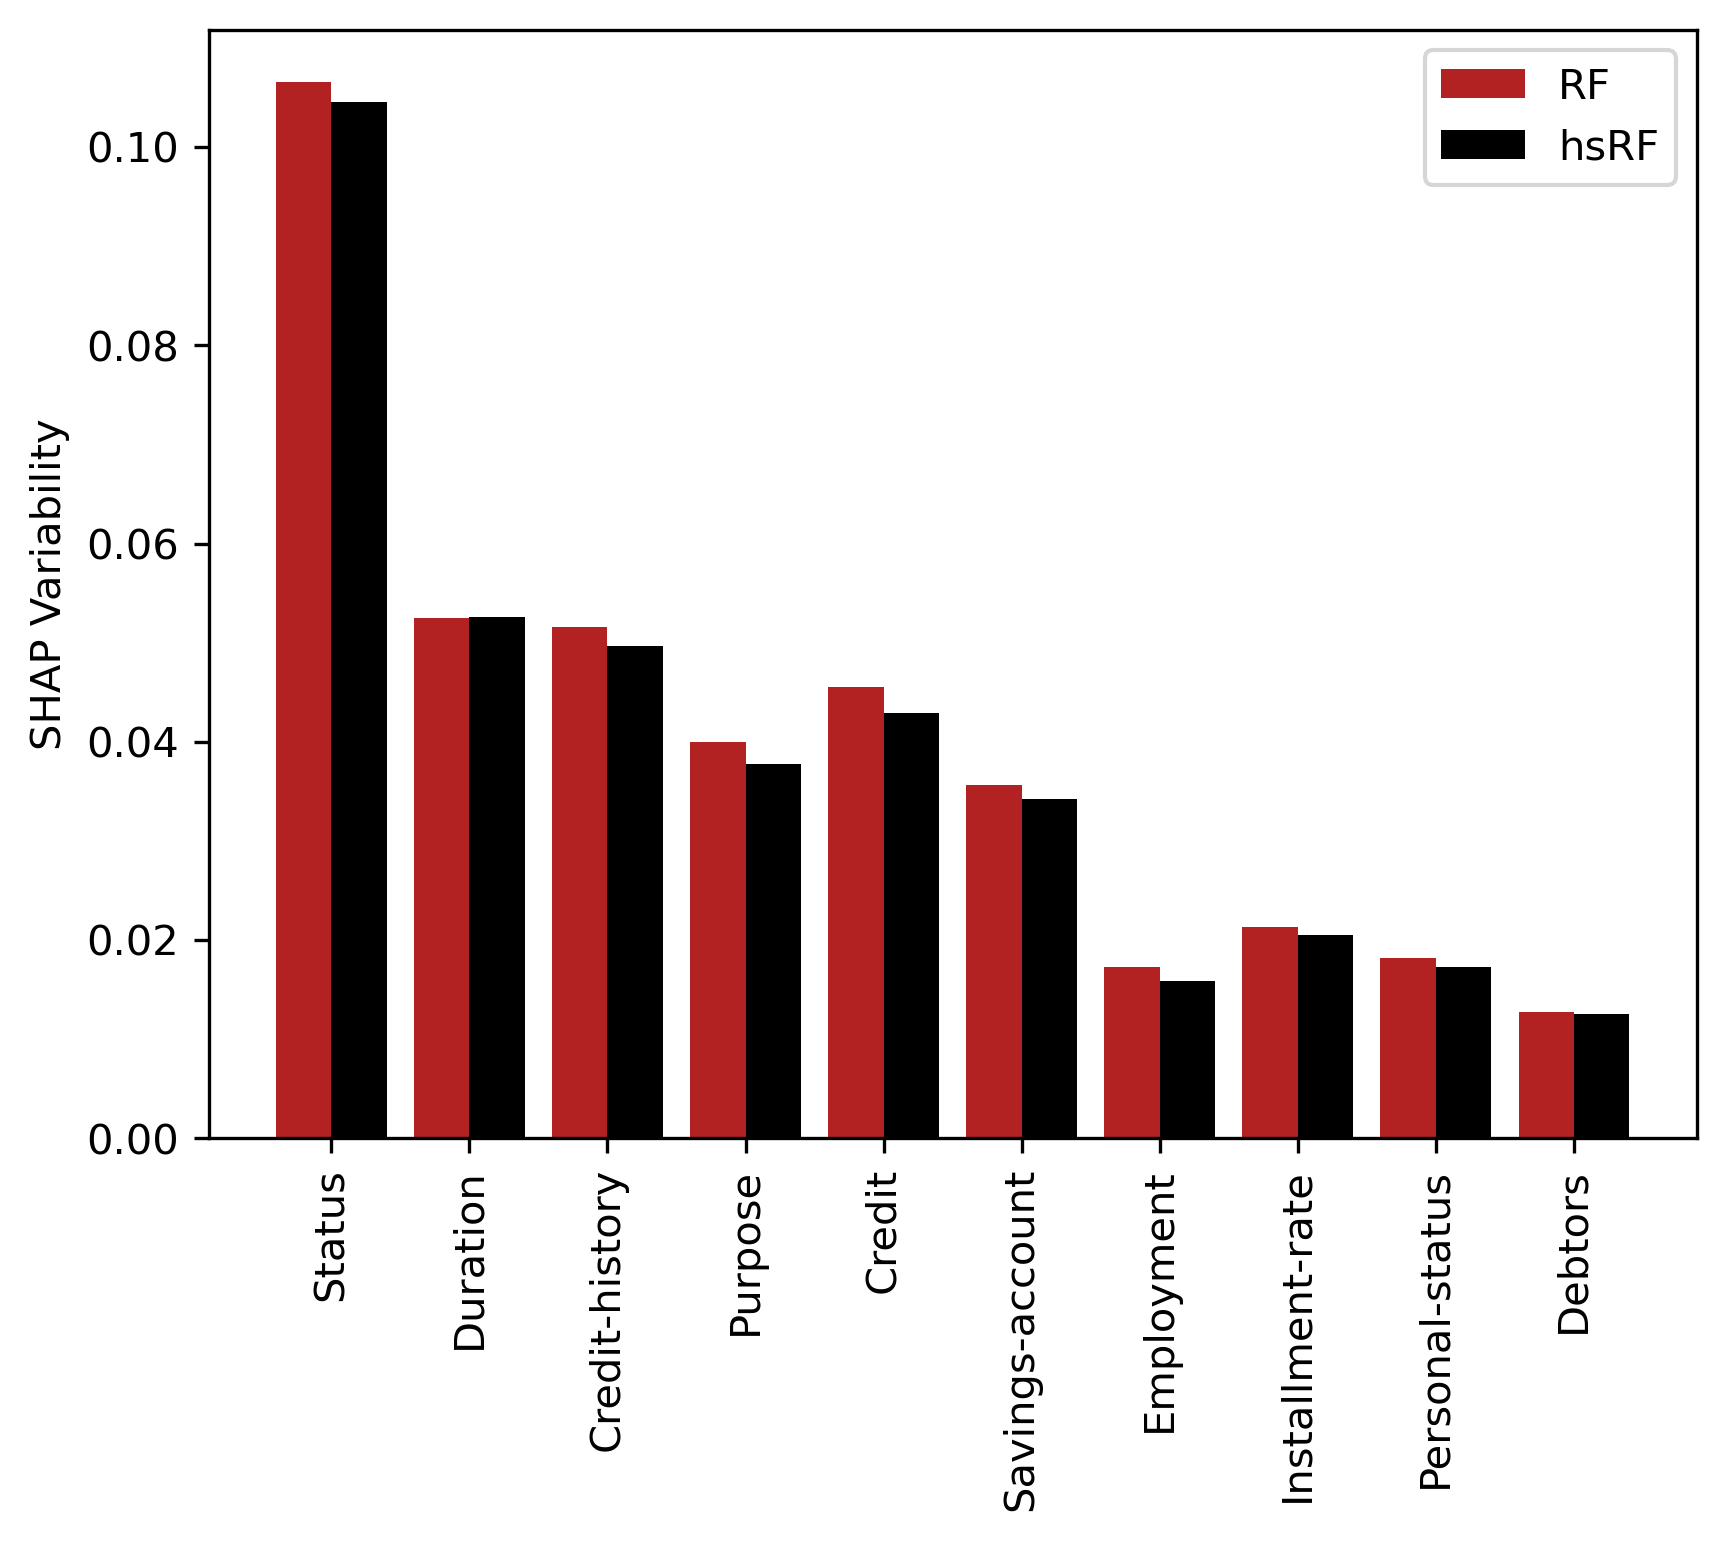
\includegraphics[width=\textwidth]{images/appendix4/SHAP_variability/german.png}
        \caption{German credit}
    \end{subfigure}
    \caption{Comparison of SHAP value variabilities for the first six classification data sets before and after applying HS.}
    \label{fig:apx4-svar1}
\end{figure}

\begin{figure}[hbt]
    \centering
    \begin{subfigure}[t]{0.45\textwidth}
        \vskip 0pt
        \centering
        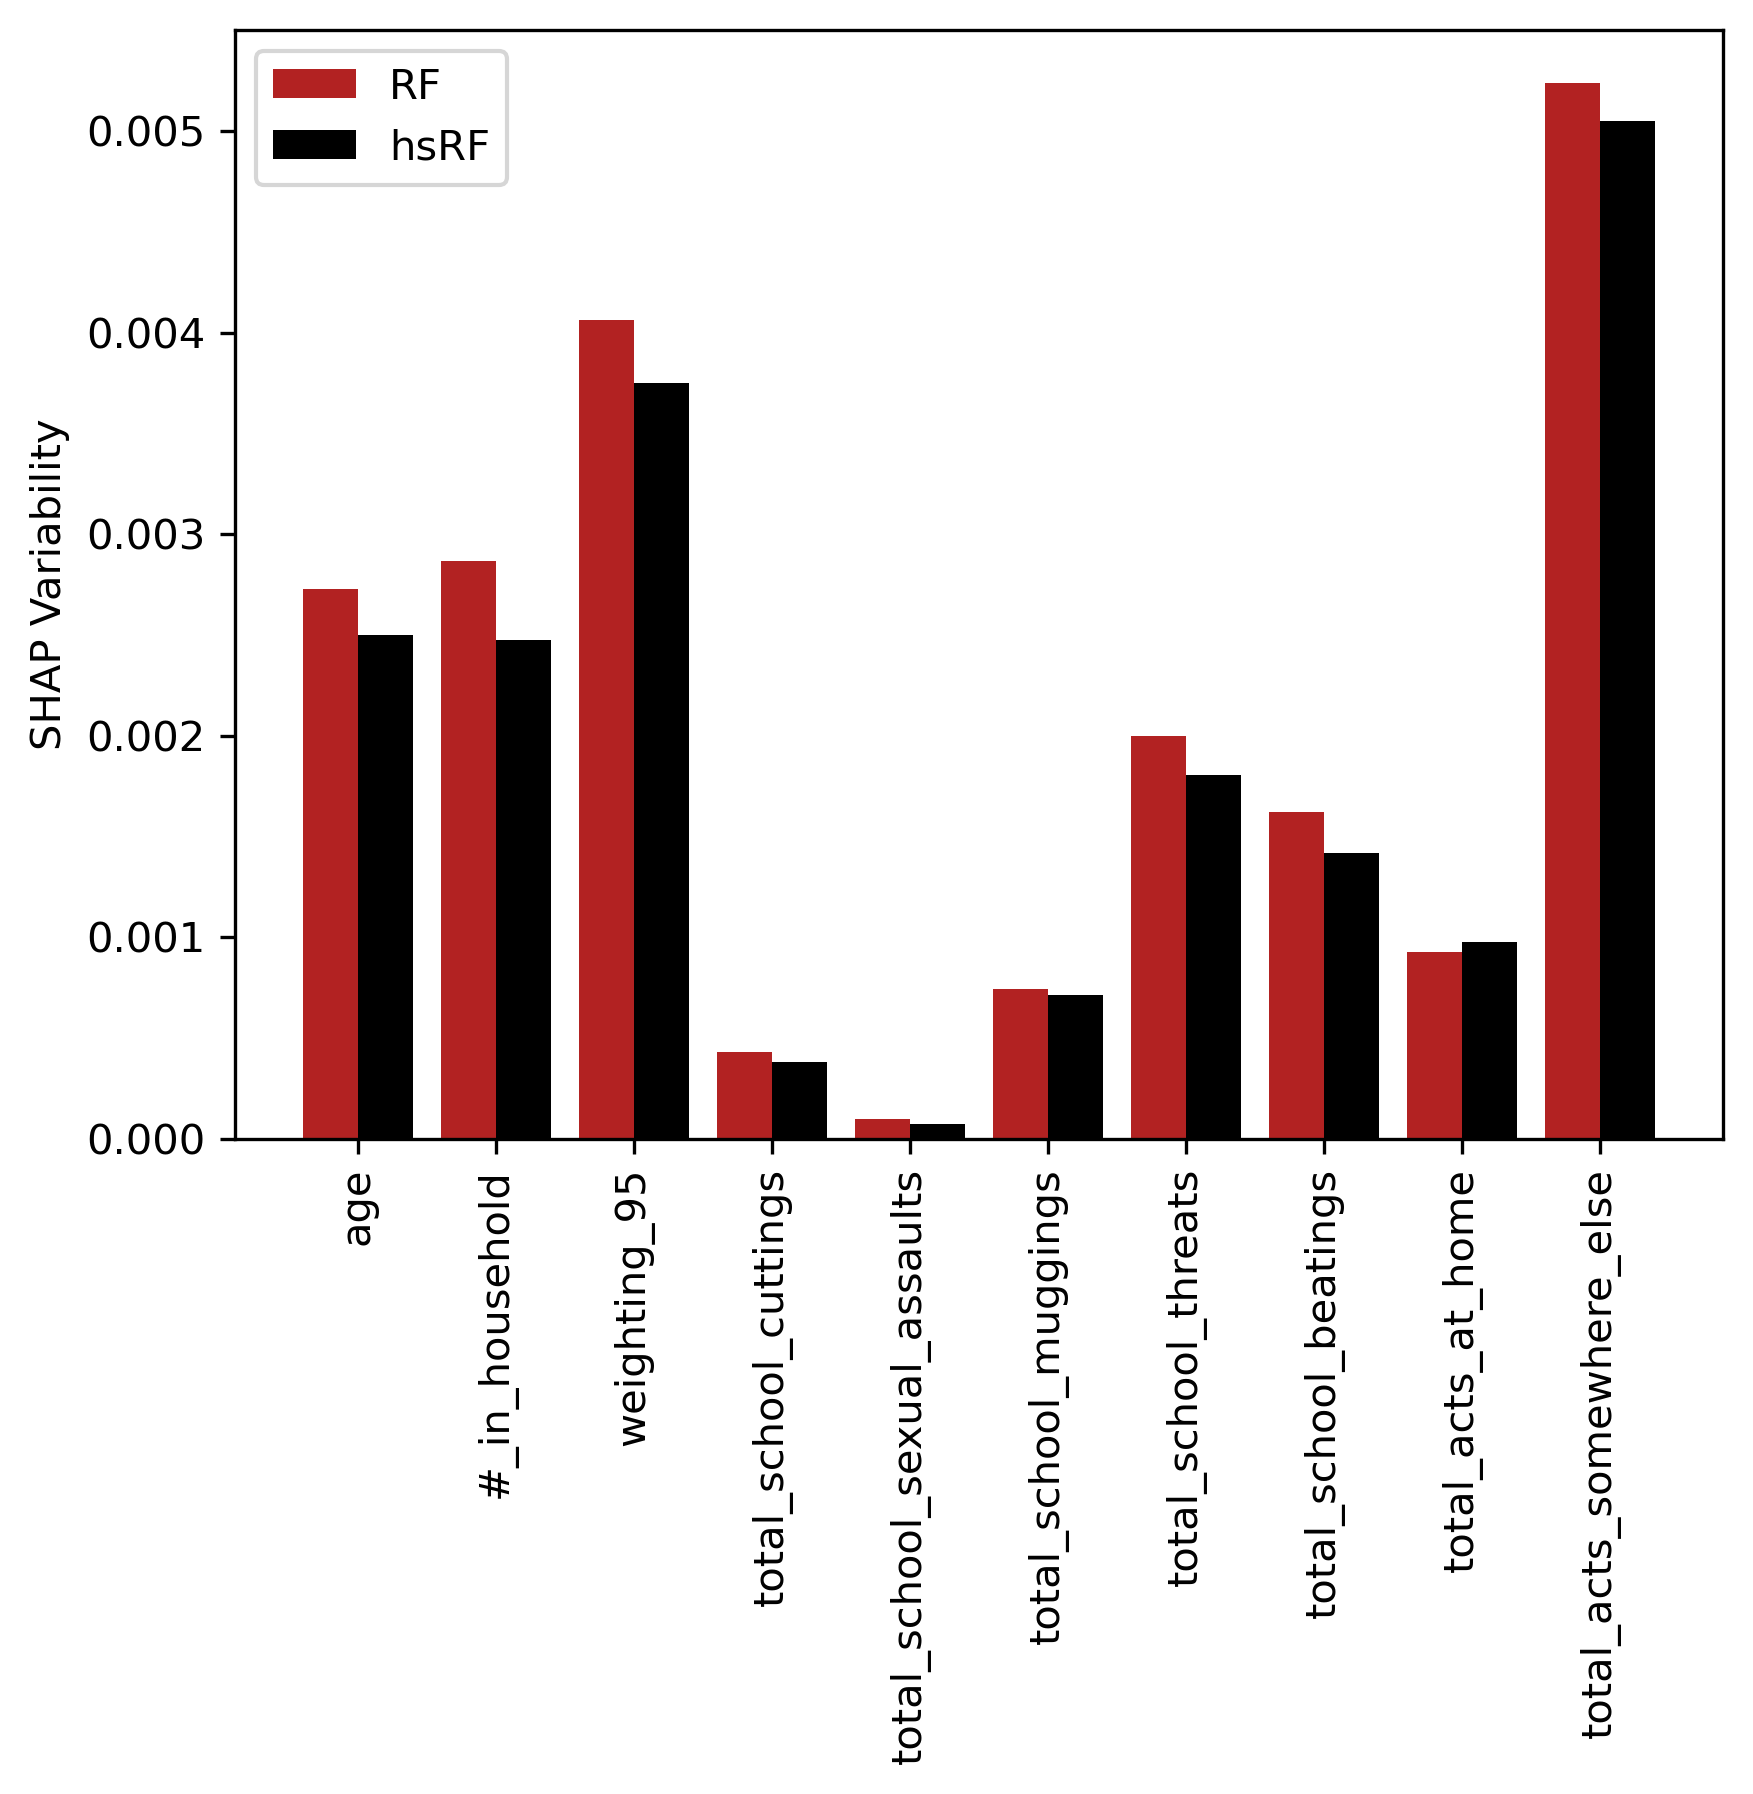
\includegraphics[width=\textwidth]{images/appendix4/SHAP_variability/juvenile_clean.png}
        \caption{Juvenile}
    \end{subfigure}
    \begin{subfigure}[t]{0.45\textwidth}
        \vskip 0pt
        \centering
        \includegraphics[width=\textwidth]{images/appendix4/SHAP_variability/compas_two_year_clean.png}
        \caption{Recidivism}
    \end{subfigure}
    \caption{Comparison of SHAP value variabilities for the last two classification data sets before and after applying HS.}
    \label{fig:apx4-svar2}
\end{figure}